\documentclass[a4paper,twocolumn,10pt]{ltjsarticle}
\usepackage{luatexja-fontspec}
\setmainfont{TeX Gyre Termes}
\setmainjfont{Noto Serif CJK JP}
\setsansjfont{Noto Sans CJK JP}
\usepackage{amsmath,amssymb,bm}
\usepackage{graphicx}
\usepackage{rotating}
\usepackage{booktabs,array}
\newcolumntype{L}[1]{>{\raggedright\arraybackslash}p{#1}}
\usepackage[margin=16mm,columnsep=6.5mm]{geometry}
\usepackage{caption}
\captionsetup{font=small,labelsep=quad}
\usepackage[hidelinks]{hyperref}
\hypersetup{pdfauthor={Qu0rise},pdftitle={SoftTwin: 見た目が同じでも中身が違う食品を力センサのない柔らかい指で壊さずにつかむ},pdfsubject={Physical AI 講座 2026 応用編1 最終課題}}
\usepackage{enumitem}
\usepackage{xcolor}
\setlist{nosep,leftmargin=1.4em}
\graphicspath{{../figures/}}
\renewcommand{\figurename}{図}
\renewcommand{\tablename}{表}
\definecolor{prop}{HTML}{2A78D6}
\definecolor{crit}{HTML}{D03B3B}
% numbers come from results/metrics.json via scripts/make_numbers.py (never typed by hand)
\makeatletter
\newcommand{\V}[1]{\@ifundefined{V@#1}{\textcolor{red}{??#1}}{\csname V@#1\endcsname}}
\makeatother
% generated by scripts/make_numbers.py from results/*.json -- do not edit
\expandafter\def\csname V@act.gbplay\endcsname{1.2}
\expandafter\def\csname V@act.gbplay.bias\endcsname{-0.3}
\expandafter\def\csname V@act.gbplay.gbias\endcsname{-0.3}
\expandafter\def\csname V@act.gbplay.grip\endcsname{0.8}
\expandafter\def\csname V@act.greybox\endcsname{1.9}
\expandafter\def\csname V@act.greybox.bias\endcsname{-0.5}
\expandafter\def\csname V@act.greybox.gbias\endcsname{+1.1}
\expandafter\def\csname V@act.greybox.grip\endcsname{1.7}
\expandafter\def\csname V@act.learned\endcsname{2.4}
\expandafter\def\csname V@act.learned.bias\endcsname{-1.8}
\expandafter\def\csname V@act.learned.gbias\endcsname{-1.3}
\expandafter\def\csname V@act.learned.grip\endcsname{2.3}
\expandafter\def\csname V@act.linear\endcsname{13.6}
\expandafter\def\csname V@act.linear.bias\endcsname{-11.5}
\expandafter\def\csname V@act.linear.gbias\endcsname{-7.8}
\expandafter\def\csname V@act.linear.grip\endcsname{15.9}
\expandafter\def\csname V@act.static\endcsname{9.0}
\expandafter\def\csname V@act.static.bias\endcsname{-1.7}
\expandafter\def\csname V@act.static.gbias\endcsname{+2.2}
\expandafter\def\csname V@act.static.grip\endcsname{10.3}
\expandafter\def\csname V@cal.mj.maxdev\endcsname{1\,\%}
\expandafter\def\csname V@cal.px.range\endcsname{0.96〜0.99}
\expandafter\def\csname V@ctl.dFdp\endcsname{0.25}
\expandafter\def\csname V@ctl.rise22\endcsname{1.9〜2.2}
\expandafter\def\csname V@ctl.taucl\endcsname{1.0}
\expandafter\def\csname V@cv.all\endcsname{100.0$\pm$0.0}
\expandafter\def\csname V@cv.finger\endcsname{76.9$\pm$7.6}
\expandafter\def\csname V@cv.plunger\endcsname{99.8$\pm$0.5}
\expandafter\def\csname V@cv.vision\endcsname{67.9$\pm$6.2}
\expandafter\def\csname V@ds.min\endcsname{3.8}
\expandafter\def\csname V@ds.n\endcsname{420}
\expandafter\def\csname V@ds.outcomes\endcsname{成功 45\,\%・破損 22\,\%・滑り 14\,\%・落下 19\,\%}
\expandafter\def\csname V@ds.samples\endcsname{156,423}
\expandafter\def\csname V@env.mujoco\endcsname{3.15.0}
\expandafter\def\csname V@fail.common\endcsname{17}
\expandafter\def\csname V@fail.margin.strawberry_overripe.fail\endcsname{2.9}
\expandafter\def\csname V@fail.margin.strawberry_overripe.ok\endcsname{3.3}
\expandafter\def\csname V@fail.margin.tofu.fail\endcsname{2.0}
\expandafter\def\csname V@fail.margin.tofu.ok\endcsname{2.3}
\expandafter\def\csname V@fail.margin.tomato_overripe.fail\endcsname{1.6}
\expandafter\def\csname V@fail.margin.tomato_overripe.ok\endcsname{2.0}
\expandafter\def\csname V@fail.mass.strawberry_overripe.fail\endcsname{21}
\expandafter\def\csname V@fail.mass.strawberry_overripe.ok\endcsname{19}
\expandafter\def\csname V@fail.mass.tofu.fail\endcsname{37}
\expandafter\def\csname V@fail.mass.tofu.ok\endcsname{35}
\expandafter\def\csname V@fail.mass.tomato_overripe.fail\endcsname{48}
\expandafter\def\csname V@fail.mass.tomato_overripe.ok\endcsname{43}
\expandafter\def\csname V@fail.massv.bolt\endcsname{0}
\expandafter\def\csname V@fail.massv.egg\endcsname{0}
\expandafter\def\csname V@fail.massv.strawberry\endcsname{0}
\expandafter\def\csname V@fail.massv.strawberry_overripe\endcsname{6}
\expandafter\def\csname V@fail.massv.tofu\endcsname{1}
\expandafter\def\csname V@fail.massv.tomato\endcsname{0}
\expandafter\def\csname V@fail.massv.tomato_overripe\endcsname{6}
\expandafter\def\csname V@fail.mu.strawberry_overripe.fail\endcsname{0.55}
\expandafter\def\csname V@fail.mu.strawberry_overripe.ok\endcsname{0.59}
\expandafter\def\csname V@fail.mu.tofu.fail\endcsname{0.37}
\expandafter\def\csname V@fail.mu.tofu.ok\endcsname{0.41}
\expandafter\def\csname V@fail.mu.tomato_overripe.fail\endcsname{0.51}
\expandafter\def\csname V@fail.mu.tomato_overripe.ok\endcsname{0.60}
\expandafter\def\csname V@fail.oracle.bolt\endcsname{0}
\expandafter\def\csname V@fail.oracle.bolt.cr\endcsname{0}
\expandafter\def\csname V@fail.oracle.egg\endcsname{0}
\expandafter\def\csname V@fail.oracle.egg.cr\endcsname{0}
\expandafter\def\csname V@fail.oracle.strawberry\endcsname{0}
\expandafter\def\csname V@fail.oracle.strawberry.cr\endcsname{0}
\expandafter\def\csname V@fail.oracle.strawberry_overripe\endcsname{6}
\expandafter\def\csname V@fail.oracle.strawberry_overripe.cr\endcsname{0}
\expandafter\def\csname V@fail.oracle.tofu\endcsname{3}
\expandafter\def\csname V@fail.oracle.tofu.cr\endcsname{0}
\expandafter\def\csname V@fail.oracle.tomato\endcsname{0}
\expandafter\def\csname V@fail.oracle.tomato.cr\endcsname{0}
\expandafter\def\csname V@fail.oracle.tomato_overripe\endcsname{8}
\expandafter\def\csname V@fail.oracle.tomato_overripe.cr\endcsname{0}
\expandafter\def\csname V@fail.plunger.bolt\endcsname{0}
\expandafter\def\csname V@fail.plunger.bolt.cr\endcsname{0}
\expandafter\def\csname V@fail.plunger.egg\endcsname{0}
\expandafter\def\csname V@fail.plunger.egg.cr\endcsname{0}
\expandafter\def\csname V@fail.plunger.firmer\endcsname{0}
\expandafter\def\csname V@fail.plunger.n\endcsname{17}
\expandafter\def\csname V@fail.plunger.strawberry\endcsname{0}
\expandafter\def\csname V@fail.plunger.strawberry.cr\endcsname{0}
\expandafter\def\csname V@fail.plunger.strawberry_overripe\endcsname{6}
\expandafter\def\csname V@fail.plunger.strawberry_overripe.cr\endcsname{0}
\expandafter\def\csname V@fail.plunger.tofu\endcsname{3}
\expandafter\def\csname V@fail.plunger.tofu.cr\endcsname{0}
\expandafter\def\csname V@fail.plunger.tomato\endcsname{0}
\expandafter\def\csname V@fail.plunger.tomato.cr\endcsname{0}
\expandafter\def\csname V@fail.plunger.tomato_overripe\endcsname{8}
\expandafter\def\csname V@fail.plunger.tomato_overripe.cr\endcsname{0}
\expandafter\def\csname V@fail.prior.firmer\endcsname{60}
\expandafter\def\csname V@fail.prior.n\endcsname{63}
\expandafter\def\csname V@ho.q1.affine.cr\endcsname{32}
\expandafter\def\csname V@ho.q1.affine.succ\endcsname{58.0}
\expandafter\def\csname V@ho.q1.gbplay.cr\endcsname{0}
\expandafter\def\csname V@ho.q1.gbplay.succ\endcsname{94.7}
\expandafter\def\csname V@ho.q1.greybox.cr\endcsname{0}
\expandafter\def\csname V@ho.q1.greybox.succ\endcsname{90.7}
\expandafter\def\csname V@ho.q1.ideal.cr\endcsname{0}
\expandafter\def\csname V@ho.q1.ideal.succ\endcsname{96.7}
\expandafter\def\csname V@ho.q1.learned.cr\endcsname{0}
\expandafter\def\csname V@ho.q1.learned.succ\endcsname{94.7}
\expandafter\def\csname V@ho.q1.n\endcsname{150}
\expandafter\def\csname V@ho.q1.recipe.cr\endcsname{0}
\expandafter\def\csname V@ho.q1.recipe.succ\endcsname{97.3}
\expandafter\def\csname V@ho.q1.static.cr\endcsname{0}
\expandafter\def\csname V@ho.q1.static.succ\endcsname{92.0}
\expandafter\def\csname V@ho.q1.tip.cr\endcsname{0}
\expandafter\def\csname V@ho.q1.tip.succ\endcsname{98.0}
\expandafter\def\csname V@ho.q2.finger.cr\endcsname{20}
\expandafter\def\csname V@ho.q2.finger.la\endcsname{46.7}
\expandafter\def\csname V@ho.q2.finger.la.ci\endcsname{[34.6, 59.1]}
\expandafter\def\csname V@ho.q2.finger.la.cr\endcsname{19}
\expandafter\def\csname V@ho.q2.finger.succ\endcsname{81.4}
\expandafter\def\csname V@ho.q2.fw.cr\endcsname{0}
\expandafter\def\csname V@ho.q2.fw.la\endcsname{75.0}
\expandafter\def\csname V@ho.q2.fw.la.ci\endcsname{[62.8, 84.2]}
\expandafter\def\csname V@ho.q2.fw.la.cr\endcsname{0}
\expandafter\def\csname V@ho.q2.fw.succ\endcsname{91.4}
\expandafter\def\csname V@ho.q2.fwloo.cr\endcsname{85}
\expandafter\def\csname V@ho.q2.fwloo.la\endcsname{6.7}
\expandafter\def\csname V@ho.q2.fwloo.la.ci\endcsname{[2.6, 15.9]}
\expandafter\def\csname V@ho.q2.fwloo.la.cr\endcsname{56}
\expandafter\def\csname V@ho.q2.fwloo.succ\endcsname{59.5}
\expandafter\def\csname V@ho.q2.mass.cr\endcsname{0}
\expandafter\def\csname V@ho.q2.mass.la\endcsname{88.3}
\expandafter\def\csname V@ho.q2.mass.la.ci\endcsname{[77.8, 94.2]}
\expandafter\def\csname V@ho.q2.mass.la.cr\endcsname{0}
\expandafter\def\csname V@ho.q2.mass.succ\endcsname{94.8}
\expandafter\def\csname V@ho.q2.oracle.cr\endcsname{0}
\expandafter\def\csname V@ho.q2.oracle.la\endcsname{81.7}
\expandafter\def\csname V@ho.q2.oracle.la.ci\endcsname{[70.1, 89.4]}
\expandafter\def\csname V@ho.q2.oracle.la.cr\endcsname{0}
\expandafter\def\csname V@ho.q2.oracle.succ\endcsname{93.3}
\expandafter\def\csname V@ho.q2.plunger.cr\endcsname{0}
\expandafter\def\csname V@ho.q2.plunger.la\endcsname{81.7}
\expandafter\def\csname V@ho.q2.plunger.la.ci\endcsname{[70.1, 89.4]}
\expandafter\def\csname V@ho.q2.plunger.la.cr\endcsname{0}
\expandafter\def\csname V@ho.q2.plunger.succ\endcsname{92.9}
\expandafter\def\csname V@ho.q2.prior.cr\endcsname{60}
\expandafter\def\csname V@ho.q2.prior.la\endcsname{0.0}
\expandafter\def\csname V@ho.q2.prior.la.ci\endcsname{[0.0, 6.0]}
\expandafter\def\csname V@ho.q2.prior.la.cr\endcsname{60}
\expandafter\def\csname V@ho.q2.prior.succ\endcsname{70.0}
\expandafter\def\csname V@ho.q2.soft.cr\endcsname{0}
\expandafter\def\csname V@ho.q2.soft.la\endcsname{63.3}
\expandafter\def\csname V@ho.q2.soft.la.ci\endcsname{[50.7, 74.4]}
\expandafter\def\csname V@ho.q2.soft.la.cr\endcsname{0}
\expandafter\def\csname V@ho.q2.soft.succ\endcsname{51.0}
\expandafter\def\csname V@ho.q2.tip.cr\endcsname{0}
\expandafter\def\csname V@ho.q2.tip.la\endcsname{96.7}
\expandafter\def\csname V@ho.q2.tip.la.ci\endcsname{[88.6, 99.1]}
\expandafter\def\csname V@ho.q2.tip.la.cr\endcsname{0}
\expandafter\def\csname V@ho.q2.tip.succ\endcsname{98.1}
\expandafter\def\csname V@ho.seeds\endcsname{30〜59}
\expandafter\def\csname V@pm.strawberry.finger\endcsname{60}
\expandafter\def\csname V@pm.strawberry.finger0\endcsname{82}
\expandafter\def\csname V@pm.strawberry.plunger\endcsname{100}
\expandafter\def\csname V@pm.strawberry.plunger15\endcsname{98}
\expandafter\def\csname V@pm.strawberry.plunger15n50\endcsname{90}
\expandafter\def\csname V@pm.strawberry.plunger2n50\endcsname{99}
\expandafter\def\csname V@pm.tomato.finger\endcsname{70}
\expandafter\def\csname V@pm.tomato.finger0\endcsname{85}
\expandafter\def\csname V@pm.tomato.plunger\endcsname{100}
\expandafter\def\csname V@pm.tomato.plunger15\endcsname{97}
\expandafter\def\csname V@pm.tomato.plunger15n50\endcsname{67}
\expandafter\def\csname V@pm.tomato.plunger2n50\endcsname{90}
\expandafter\def\csname V@px.affine.cr\endcsname{20}
\expandafter\def\csname V@px.affine.mae\endcsname{0.81}
\expandafter\def\csname V@px.affine.succ\endcsname{61.0}
\expandafter\def\csname V@px.greybox.cr\endcsname{0}
\expandafter\def\csname V@px.greybox.mae\endcsname{0.27}
\expandafter\def\csname V@px.greybox.succ\endcsname{98.0}
\expandafter\def\csname V@px.ideal.cr\endcsname{0}
\expandafter\def\csname V@px.ideal.mae\endcsname{0.12}
\expandafter\def\csname V@px.ideal.succ\endcsname{100.0}
\expandafter\def\csname V@px.learned.cr\endcsname{0}
\expandafter\def\csname V@px.learned.mae\endcsname{0.13}
\expandafter\def\csname V@px.learned.succ\endcsname{99.0}
\expandafter\def\csname V@px.n\endcsname{100}
\expandafter\def\csname V@px.recipe.cr\endcsname{0}
\expandafter\def\csname V@px.recipe.mae\endcsname{0.08}
\expandafter\def\csname V@px.recipe.succ\endcsname{100.0}
\expandafter\def\csname V@px.static.cr\endcsname{0}
\expandafter\def\csname V@px.static.mae\endcsname{0.33}
\expandafter\def\csname V@px.static.succ\endcsname{97.0}
\expandafter\def\csname V@px.tip.cr\endcsname{0}
\expandafter\def\csname V@px.tip.mae\endcsname{0.22}
\expandafter\def\csname V@px.tip.succ\endcsname{100.0}
\expandafter\def\csname V@q1.affine.bias\endcsname{0.69}
\expandafter\def\csname V@q1.affine.bolt.slip\endcsname{30}
\expandafter\def\csname V@q1.affine.ci\endcsname{[50.0, 65.6]}
\expandafter\def\csname V@q1.affine.cr\endcsname{33}
\expandafter\def\csname V@q1.affine.eggdrop\endcsname{0}
\expandafter\def\csname V@q1.affine.hold\endcsname{1.42}
\expandafter\def\csname V@q1.affine.mae\endcsname{1.10}
\expandafter\def\csname V@q1.affine.succ\endcsname{58.0}
\expandafter\def\csname V@q1.affine.tofudrop\endcsname{0}
\expandafter\def\csname V@q1.gbplay.bias\endcsname{1.06}
\expandafter\def\csname V@q1.gbplay.ci\endcsname{[89.8, 97.3]}
\expandafter\def\csname V@q1.gbplay.cr\endcsname{0}
\expandafter\def\csname V@q1.gbplay.eggdrop\endcsname{0}
\expandafter\def\csname V@q1.gbplay.fberr\endcsname{+0.4}
\expandafter\def\csname V@q1.gbplay.hold\endcsname{0.94}
\expandafter\def\csname V@q1.gbplay.mae\endcsname{0.15}
\expandafter\def\csname V@q1.gbplay.succ\endcsname{94.7}
\expandafter\def\csname V@q1.gbplay.tofudrop\endcsname{8}
\expandafter\def\csname V@q1.greybox.bias\endcsname{1.14}
\expandafter\def\csname V@q1.greybox.ci\endcsname{[84.9, 94.4]}
\expandafter\def\csname V@q1.greybox.cr\endcsname{0}
\expandafter\def\csname V@q1.greybox.eggdrop\endcsname{1}
\expandafter\def\csname V@q1.greybox.hold\endcsname{0.89}
\expandafter\def\csname V@q1.greybox.mae\endcsname{0.27}
\expandafter\def\csname V@q1.greybox.succ\endcsname{90.7}
\expandafter\def\csname V@q1.greybox.tofudrop\endcsname{13}
\expandafter\def\csname V@q1.ideal.bias\endcsname{1.03}
\expandafter\def\csname V@q1.ideal.ci\endcsname{[93.3, 99.0]}
\expandafter\def\csname V@q1.ideal.cr\endcsname{0}
\expandafter\def\csname V@q1.ideal.eggdrop\endcsname{0}
\expandafter\def\csname V@q1.ideal.hold\endcsname{0.99}
\expandafter\def\csname V@q1.ideal.mae\endcsname{0.14}
\expandafter\def\csname V@q1.ideal.succ\endcsname{97.3}
\expandafter\def\csname V@q1.ideal.tofudrop\endcsname{4}
\expandafter\def\csname V@q1.learned.bias\endcsname{1.04}
\expandafter\def\csname V@q1.learned.ci\endcsname{[91.5, 98.2]}
\expandafter\def\csname V@q1.learned.cr\endcsname{0}
\expandafter\def\csname V@q1.learned.eggdrop\endcsname{0}
\expandafter\def\csname V@q1.learned.hold\endcsname{0.97}
\expandafter\def\csname V@q1.learned.mae\endcsname{0.14}
\expandafter\def\csname V@q1.learned.succ\endcsname{96.0}
\expandafter\def\csname V@q1.learned.tofudrop\endcsname{6}
\expandafter\def\csname V@q1.n\endcsname{150}
\expandafter\def\csname V@q1.recipe.bias\endcsname{1.01}
\expandafter\def\csname V@q1.recipe.ci\endcsname{[94.3, 99.3]}
\expandafter\def\csname V@q1.recipe.cr\endcsname{0}
\expandafter\def\csname V@q1.recipe.eggdrop\endcsname{0}
\expandafter\def\csname V@q1.recipe.hold\endcsname{1.01}
\expandafter\def\csname V@q1.recipe.mae\endcsname{0.10}
\expandafter\def\csname V@q1.recipe.succ\endcsname{98.0}
\expandafter\def\csname V@q1.recipe.tofudrop\endcsname{3}
\expandafter\def\csname V@q1.static.bias\endcsname{1.16}
\expandafter\def\csname V@q1.static.ci\endcsname{[84.2, 93.8]}
\expandafter\def\csname V@q1.static.cr\endcsname{0}
\expandafter\def\csname V@q1.static.eggdrop\endcsname{2}
\expandafter\def\csname V@q1.static.hold\endcsname{0.88}
\expandafter\def\csname V@q1.static.mae\endcsname{0.33}
\expandafter\def\csname V@q1.static.succ\endcsname{90.0}
\expandafter\def\csname V@q1.static.tofudrop\endcsname{13}
\expandafter\def\csname V@q1.tip.bias\endcsname{0.91}
\expandafter\def\csname V@q1.tip.ci\endcsname{[95.3, 99.6]}
\expandafter\def\csname V@q1.tip.cr\endcsname{0}
\expandafter\def\csname V@q1.tip.eggdrop\endcsname{0}
\expandafter\def\csname V@q1.tip.hold\endcsname{1.09}
\expandafter\def\csname V@q1.tip.mae\endcsname{0.26}
\expandafter\def\csname V@q1.tip.succ\endcsname{98.7}
\expandafter\def\csname V@q1.tip.tofudrop\endcsname{2}
\expandafter\def\csname V@q2.ct.delta\endcsname{4.5}
\expandafter\def\csname V@q2.finger.cr\endcsname{10}
\expandafter\def\csname V@q2.finger.ct\endcsname{11.8}
\expandafter\def\csname V@q2.finger.la\endcsname{56.7}
\expandafter\def\csname V@q2.finger.la.cr\endcsname{10}
\expandafter\def\csname V@q2.finger.succ\endcsname{82.9}
\expandafter\def\csname V@q2.fw.cr\endcsname{0}
\expandafter\def\csname V@q2.fw.ct\endcsname{16.0}
\expandafter\def\csname V@q2.fw.la\endcsname{66.7}
\expandafter\def\csname V@q2.fw.la.cr\endcsname{0}
\expandafter\def\csname V@q2.fw.succ\endcsname{90.5}
\expandafter\def\csname V@q2.fwloo.cr\endcsname{81}
\expandafter\def\csname V@q2.fwloo.ct\endcsname{16.4}
\expandafter\def\csname V@q2.fwloo.la\endcsname{11.7}
\expandafter\def\csname V@q2.fwloo.la.cr\endcsname{52}
\expandafter\def\csname V@q2.fwloo.succ\endcsname{61.0}
\expandafter\def\csname V@q2.mass.cr\endcsname{0}
\expandafter\def\csname V@q2.mass.ct\endcsname{16.1}
\expandafter\def\csname V@q2.mass.la\endcsname{80.0}
\expandafter\def\csname V@q2.mass.la.cr\endcsname{0}
\expandafter\def\csname V@q2.mass.succ\endcsname{93.8}
\expandafter\def\csname V@q2.oracle.cr\endcsname{0}
\expandafter\def\csname V@q2.oracle.ct\endcsname{11.1}
\expandafter\def\csname V@q2.oracle.la\endcsname{76.7}
\expandafter\def\csname V@q2.oracle.la.cr\endcsname{0}
\expandafter\def\csname V@q2.oracle.succ\endcsname{91.9}
\expandafter\def\csname V@q2.plunger.cr\endcsname{0}
\expandafter\def\csname V@q2.plunger.ct\endcsname{16.1}
\expandafter\def\csname V@q2.plunger.la\endcsname{76.7}
\expandafter\def\csname V@q2.plunger.la.cr\endcsname{0}
\expandafter\def\csname V@q2.plunger.succ\endcsname{91.9}
\expandafter\def\csname V@q2.prior.cr\endcsname{60}
\expandafter\def\csname V@q2.prior.ct\endcsname{11.5}
\expandafter\def\csname V@q2.prior.la\endcsname{0.0}
\expandafter\def\csname V@q2.prior.la.cr\endcsname{60}
\expandafter\def\csname V@q2.prior.succ\endcsname{70.0}
\expandafter\def\csname V@q2.soft.cr\endcsname{0}
\expandafter\def\csname V@q2.soft.ct\endcsname{9.9}
\expandafter\def\csname V@q2.soft.la\endcsname{58.3}
\expandafter\def\csname V@q2.soft.la.cr\endcsname{0}
\expandafter\def\csname V@q2.soft.succ\endcsname{46.2}
\expandafter\def\csname V@q2.tip.cr\endcsname{1}
\expandafter\def\csname V@q2.tip.ct\endcsname{16.5}
\expandafter\def\csname V@q2.tip.la\endcsname{91.7}
\expandafter\def\csname V@q2.tip.la.cr\endcsname{1}
\expandafter\def\csname V@q2.tip.succ\endcsname{97.1}
\expandafter\def\csname V@rec.hi\endcsname{24}
\expandafter\def\csname V@rec.lo\endcsname{15}
\expandafter\def\csname V@req.R1\endcsname{2.40° \checkmark}
\expandafter\def\csname V@req.R2\endcsname{0.14\,N \checkmark}
\expandafter\def\csname V@req.R3\endcsname{96.0 [91.5, 98.2] \checkmark}
\expandafter\def\csname V@req.R4\endcsname{0.0 [0.0, 2.5] \checkmark}
\expandafter\def\csname V@req.R5\endcsname{76.7 [64.6, 85.6] \textcolor{crit}{未達}}
\expandafter\def\csname V@req.R6\endcsname{0.0 [0.0, 1.8] \checkmark}
\expandafter\def\csname V@req.R7\endcsname{99.8 \checkmark}
\expandafter\def\csname V@req.R8\endcsname{98.0 \checkmark}
\expandafter\def\csname V@rob.kb080.max\endcsname{88}
\expandafter\def\csname V@rob.kb080.min\endcsname{76}
\expandafter\def\csname V@rob.kb100.pk\endcsname{1.01}
\expandafter\def\csname V@rob.kb125.cr\endcsname{0}
\expandafter\def\csname V@rob.kb125.greybox.cr\endcsname{0}
\expandafter\def\csname V@rob.kb125.greybox.pk\endcsname{1.13}
\expandafter\def\csname V@rob.kb125.learned.pk\endcsname{1.26}
\expandafter\def\csname V@rob.kb125.pk\endcsname{1.26}
\expandafter\def\csname V@rob.kb125.recipe.cr\endcsname{0}
\expandafter\def\csname V@rob.kb125.recipe.pk\endcsname{1.30}
\expandafter\def\csname V@rob.kb125.static.cr\endcsname{0}
\expandafter\def\csname V@rob.kb125.static.pk\endcsname{1.13}
\expandafter\def\csname V@rob.kb125cal.cr\endcsname{1}
\expandafter\def\csname V@rob.kb125cal.pk\endcsname{1.35}
\expandafter\def\csname V@rob.learned.20\endcsname{92}
\expandafter\def\csname V@rob.learned.30\endcsname{80}
\expandafter\def\csname V@rob.learned.30.cr\endcsname{4}
\expandafter\def\csname V@rob.learnedcal.20\endcsname{98}
\expandafter\def\csname V@rob.learnedcal.30\endcsname{94}
\expandafter\def\csname V@rob.learnedcal.30.cr\endcsname{2}
\expandafter\def\csname V@rob.nominal.learned\endcsname{98}
\expandafter\def\csname V@rob.nominal.learned.pk\endcsname{1.01}
\expandafter\def\csname V@rob.nominalcal.learned.pk\endcsname{1.09}
\expandafter\def\csname V@rob.recipe.30\endcsname{90}
\expandafter\def\csname V@rob.recipe.30.cr\endcsname{3}
\expandafter\def\csname V@s2s.affine.crsame\endcsname{98/100}
\expandafter\def\csname V@s2s.affine.kappa\endcsname{0.95}
\expandafter\def\csname V@s2s.affine.mj\endcsname{58.0}
\expandafter\def\csname V@s2s.affine.pk.mj\endcsname{3.41}
\expandafter\def\csname V@s2s.affine.pk.px\endcsname{3.31}
\expandafter\def\csname V@s2s.affine.px\endcsname{61.0}
\expandafter\def\csname V@s2s.affine.rel.soft\endcsname{1.0}
\expandafter\def\csname V@s2s.affine.rel.stiff\endcsname{14}
\expandafter\def\csname V@s2s.affine.same\endcsname{97/100}
\expandafter\def\csname V@s2s.all.same\endcsname{658/700}
\expandafter\def\csname V@s2s.diff.n\endcsname{42}
\expandafter\def\csname V@s2s.diff.tofu\endcsname{30}
\expandafter\def\csname V@s2s.greybox.crsame\endcsname{100/100}
\expandafter\def\csname V@s2s.greybox.kappa\endcsname{-0.04}
\expandafter\def\csname V@s2s.greybox.mj\endcsname{89.0}
\expandafter\def\csname V@s2s.greybox.pk.mj\endcsname{2.02}
\expandafter\def\csname V@s2s.greybox.pk.px\endcsname{1.98}
\expandafter\def\csname V@s2s.greybox.px\endcsname{98.0}
\expandafter\def\csname V@s2s.greybox.rel.soft\endcsname{1.2}
\expandafter\def\csname V@s2s.greybox.rel.stiff\endcsname{24}
\expandafter\def\csname V@s2s.greybox.same\endcsname{87/100}
\expandafter\def\csname V@s2s.ideal.crsame\endcsname{100/100}
\expandafter\def\csname V@s2s.ideal.kappa\endcsname{0.00}
\expandafter\def\csname V@s2s.ideal.mj\endcsname{97.0}
\expandafter\def\csname V@s2s.ideal.pk.mj\endcsname{2.25}
\expandafter\def\csname V@s2s.ideal.pk.px\endcsname{2.25}
\expandafter\def\csname V@s2s.ideal.px\endcsname{100.0}
\expandafter\def\csname V@s2s.ideal.rel.soft\endcsname{0.5}
\expandafter\def\csname V@s2s.ideal.rel.stiff\endcsname{23}
\expandafter\def\csname V@s2s.ideal.same\endcsname{97/100}
\expandafter\def\csname V@s2s.learned.crsame\endcsname{100/100}
\expandafter\def\csname V@s2s.learned.kappa\endcsname{-0.02}
\expandafter\def\csname V@s2s.learned.mj\endcsname{96.0}
\expandafter\def\csname V@s2s.learned.pk.mj\endcsname{2.21}
\expandafter\def\csname V@s2s.learned.pk.px\endcsname{2.22}
\expandafter\def\csname V@s2s.learned.px\endcsname{99.0}
\expandafter\def\csname V@s2s.learned.rel.soft\endcsname{1.1}
\expandafter\def\csname V@s2s.learned.rel.stiff\endcsname{22}
\expandafter\def\csname V@s2s.learned.same\endcsname{95/100}
\expandafter\def\csname V@s2s.recipe.crsame\endcsname{100/100}
\expandafter\def\csname V@s2s.recipe.kappa\endcsname{0.00}
\expandafter\def\csname V@s2s.recipe.mj\endcsname{98.0}
\expandafter\def\csname V@s2s.recipe.pk.mj\endcsname{2.36}
\expandafter\def\csname V@s2s.recipe.pk.px\endcsname{2.28}
\expandafter\def\csname V@s2s.recipe.px\endcsname{100.0}
\expandafter\def\csname V@s2s.recipe.rel.soft\endcsname{0.8}
\expandafter\def\csname V@s2s.recipe.rel.stiff\endcsname{24}
\expandafter\def\csname V@s2s.recipe.same\endcsname{98/100}
\expandafter\def\csname V@s2s.static.crsame\endcsname{100/100}
\expandafter\def\csname V@s2s.static.kappa\endcsname{-0.05}
\expandafter\def\csname V@s2s.static.mj\endcsname{88.0}
\expandafter\def\csname V@s2s.static.pk.mj\endcsname{2.00}
\expandafter\def\csname V@s2s.static.pk.px\endcsname{1.98}
\expandafter\def\csname V@s2s.static.px\endcsname{97.0}
\expandafter\def\csname V@s2s.static.rel.soft\endcsname{1.3}
\expandafter\def\csname V@s2s.static.rel.stiff\endcsname{26}
\expandafter\def\csname V@s2s.static.same\endcsname{85/100}
\expandafter\def\csname V@s2s.tip.crsame\endcsname{100/100}
\expandafter\def\csname V@s2s.tip.kappa\endcsname{0.00}
\expandafter\def\csname V@s2s.tip.mj\endcsname{99.0}
\expandafter\def\csname V@s2s.tip.pk.mj\endcsname{2.50}
\expandafter\def\csname V@s2s.tip.pk.px\endcsname{2.51}
\expandafter\def\csname V@s2s.tip.px\endcsname{100.0}
\expandafter\def\csname V@s2s.tip.rel.soft\endcsname{0.7}
\expandafter\def\csname V@s2s.tip.rel.stiff\endcsname{21}
\expandafter\def\csname V@s2s.tip.same\endcsname{99/100}
\expandafter\def\csname V@split.greybox.bend_sensor\endcsname{1.001}
\expandafter\def\csname V@split.greybox.lever\endcsname{1.051}
\expandafter\def\csname V@split.greybox.muscle\endcsname{1.075}
\expandafter\def\csname V@split.greybox.n\endcsname{50}
\expandafter\def\csname V@split.greybox.skin\endcsname{1.000}
\expandafter\def\csname V@split.greybox.total\endcsname{1.138}
\expandafter\def\csname V@split.greybox_play.bend_sensor\endcsname{1.001}
\expandafter\def\csname V@split.greybox_play.lever\endcsname{1.047}
\expandafter\def\csname V@split.greybox_play.muscle\endcsname{1.013}
\expandafter\def\csname V@split.greybox_play.n\endcsname{50}
\expandafter\def\csname V@split.greybox_play.skin\endcsname{1.007}
\expandafter\def\csname V@split.greybox_play.total\endcsname{1.058}
\expandafter\def\csname V@split.learned.bend_sensor\endcsname{1.001}
\expandafter\def\csname V@split.learned.lever\endcsname{1.046}
\expandafter\def\csname V@split.learned.muscle\endcsname{0.980}
\expandafter\def\csname V@split.learned.n\endcsname{50}
\expandafter\def\csname V@split.learned.skin\endcsname{1.008}
\expandafter\def\csname V@split.learned.total\endcsname{1.041}
\expandafter\def\csname V@split.static.bend_sensor\endcsname{1.001}
\expandafter\def\csname V@split.static.lever\endcsname{1.052}
\expandafter\def\csname V@split.static.muscle\endcsname{1.101}
\expandafter\def\csname V@split.static.n\endcsname{50}
\expandafter\def\csname V@split.static.skin\endcsname{1.000}
\expandafter\def\csname V@split.static.total\endcsname{1.164}
\expandafter\def\csname V@ss.learned.0.8.cr\endcsname{0}
\expandafter\def\csname V@ss.learned.0.8.pk\endcsname{1.10}
\expandafter\def\csname V@ss.learned.0.8.strawberry.cr\endcsname{0}
\expandafter\def\csname V@ss.learned.0.8.strawberry.pk\endcsname{2.43}
\expandafter\def\csname V@ss.learned.0.8.strawberry.succ\endcsname{20/20}
\expandafter\def\csname V@ss.learned.0.8.succ\endcsname{80/80}
\expandafter\def\csname V@ss.learned.0.8.tofu.cr\endcsname{0}
\expandafter\def\csname V@ss.learned.0.8.tofu.pk\endcsname{2.48}
\expandafter\def\csname V@ss.learned.0.8.tofu.succ\endcsname{20/20}
\expandafter\def\csname V@ss.learned.0.8.tomato.cr\endcsname{0}
\expandafter\def\csname V@ss.learned.0.8.tomato.pk\endcsname{2.38}
\expandafter\def\csname V@ss.learned.0.8.tomato.succ\endcsname{20/20}
\expandafter\def\csname V@ss.learned.0.8.tomato_overripe.cr\endcsname{0}
\expandafter\def\csname V@ss.learned.0.8.tomato_overripe.pk\endcsname{1.69}
\expandafter\def\csname V@ss.learned.0.8.tomato_overripe.succ\endcsname{20/20}
\expandafter\def\csname V@ss.learned.1.2.cr\endcsname{0}
\expandafter\def\csname V@ss.learned.1.2.pk\endcsname{1.06}
\expandafter\def\csname V@ss.learned.1.2.strawberry.cr\endcsname{0}
\expandafter\def\csname V@ss.learned.1.2.strawberry.pk\endcsname{2.32}
\expandafter\def\csname V@ss.learned.1.2.strawberry.succ\endcsname{20/20}
\expandafter\def\csname V@ss.learned.1.2.succ\endcsname{46/80}
\expandafter\def\csname V@ss.learned.1.2.tofu.cr\endcsname{0}
\expandafter\def\csname V@ss.learned.1.2.tofu.pk\endcsname{2.25}
\expandafter\def\csname V@ss.learned.1.2.tofu.succ\endcsname{3/20}
\expandafter\def\csname V@ss.learned.1.2.tomato.cr\endcsname{0}
\expandafter\def\csname V@ss.learned.1.2.tomato.pk\endcsname{2.30}
\expandafter\def\csname V@ss.learned.1.2.tomato.succ\endcsname{19/20}
\expandafter\def\csname V@ss.learned.1.2.tomato_overripe.cr\endcsname{0}
\expandafter\def\csname V@ss.learned.1.2.tomato_overripe.pk\endcsname{1.70}
\expandafter\def\csname V@ss.learned.1.2.tomato_overripe.succ\endcsname{4/20}
\expandafter\def\csname V@ss.learned.1.cr\endcsname{0}
\expandafter\def\csname V@ss.learned.1.pk\endcsname{1.06}
\expandafter\def\csname V@ss.learned.1.strawberry.cr\endcsname{0}
\expandafter\def\csname V@ss.learned.1.strawberry.pk\endcsname{2.37}
\expandafter\def\csname V@ss.learned.1.strawberry.succ\endcsname{20/20}
\expandafter\def\csname V@ss.learned.1.succ\endcsname{72/80}
\expandafter\def\csname V@ss.learned.1.tofu.cr\endcsname{0}
\expandafter\def\csname V@ss.learned.1.tofu.pk\endcsname{2.32}
\expandafter\def\csname V@ss.learned.1.tofu.succ\endcsname{18/20}
\expandafter\def\csname V@ss.learned.1.tomato.cr\endcsname{0}
\expandafter\def\csname V@ss.learned.1.tomato.pk\endcsname{2.31}
\expandafter\def\csname V@ss.learned.1.tomato.succ\endcsname{20/20}
\expandafter\def\csname V@ss.learned.1.tomato_overripe.cr\endcsname{0}
\expandafter\def\csname V@ss.learned.1.tomato_overripe.pk\endcsname{1.63}
\expandafter\def\csname V@ss.learned.1.tomato_overripe.succ\endcsname{14/20}
\expandafter\def\csname V@ss.mass.0.8.cr\endcsname{0}
\expandafter\def\csname V@ss.mass.0.8.pk\endcsname{1.10}
\expandafter\def\csname V@ss.mass.0.8.strawberry.cr\endcsname{0}
\expandafter\def\csname V@ss.mass.0.8.strawberry.pk\endcsname{2.43}
\expandafter\def\csname V@ss.mass.0.8.strawberry.succ\endcsname{20/20}
\expandafter\def\csname V@ss.mass.0.8.succ\endcsname{80/80}
\expandafter\def\csname V@ss.mass.0.8.tofu.cr\endcsname{0}
\expandafter\def\csname V@ss.mass.0.8.tofu.pk\endcsname{2.48}
\expandafter\def\csname V@ss.mass.0.8.tofu.succ\endcsname{20/20}
\expandafter\def\csname V@ss.mass.0.8.tomato.cr\endcsname{0}
\expandafter\def\csname V@ss.mass.0.8.tomato.pk\endcsname{2.38}
\expandafter\def\csname V@ss.mass.0.8.tomato.succ\endcsname{20/20}
\expandafter\def\csname V@ss.mass.0.8.tomato_overripe.cr\endcsname{0}
\expandafter\def\csname V@ss.mass.0.8.tomato_overripe.pk\endcsname{1.69}
\expandafter\def\csname V@ss.mass.0.8.tomato_overripe.succ\endcsname{20/20}
\expandafter\def\csname V@ss.mass.1.2.cr\endcsname{1}
\expandafter\def\csname V@ss.mass.1.2.pk\endcsname{1.05}
\expandafter\def\csname V@ss.mass.1.2.strawberry.cr\endcsname{0}
\expandafter\def\csname V@ss.mass.1.2.strawberry.pk\endcsname{2.32}
\expandafter\def\csname V@ss.mass.1.2.strawberry.succ\endcsname{20/20}
\expandafter\def\csname V@ss.mass.1.2.succ\endcsname{54/80}
\expandafter\def\csname V@ss.mass.1.2.tofu.cr\endcsname{0}
\expandafter\def\csname V@ss.mass.1.2.tofu.pk\endcsname{2.55}
\expandafter\def\csname V@ss.mass.1.2.tofu.succ\endcsname{7/20}
\expandafter\def\csname V@ss.mass.1.2.tomato.cr\endcsname{0}
\expandafter\def\csname V@ss.mass.1.2.tomato.pk\endcsname{2.65}
\expandafter\def\csname V@ss.mass.1.2.tomato.succ\endcsname{20/20}
\expandafter\def\csname V@ss.mass.1.2.tomato_overripe.cr\endcsname{1}
\expandafter\def\csname V@ss.mass.1.2.tomato_overripe.pk\endcsname{1.88}
\expandafter\def\csname V@ss.mass.1.2.tomato_overripe.succ\endcsname{7/20}
\expandafter\def\csname V@ss.mass.1.cr\endcsname{0}
\expandafter\def\csname V@ss.mass.1.pk\endcsname{1.06}
\expandafter\def\csname V@ss.mass.1.strawberry.cr\endcsname{0}
\expandafter\def\csname V@ss.mass.1.strawberry.pk\endcsname{2.37}
\expandafter\def\csname V@ss.mass.1.strawberry.succ\endcsname{20/20}
\expandafter\def\csname V@ss.mass.1.succ\endcsname{77/80}
\expandafter\def\csname V@ss.mass.1.tofu.cr\endcsname{0}
\expandafter\def\csname V@ss.mass.1.tofu.pk\endcsname{2.53}
\expandafter\def\csname V@ss.mass.1.tofu.succ\endcsname{19/20}
\expandafter\def\csname V@ss.mass.1.tomato.cr\endcsname{0}
\expandafter\def\csname V@ss.mass.1.tomato.pk\endcsname{2.31}
\expandafter\def\csname V@ss.mass.1.tomato.succ\endcsname{20/20}
\expandafter\def\csname V@ss.mass.1.tomato_overripe.cr\endcsname{0}
\expandafter\def\csname V@ss.mass.1.tomato_overripe.pk\endcsname{1.80}
\expandafter\def\csname V@ss.mass.1.tomato_overripe.succ\endcsname{18/20}
\expandafter\def\csname V@ss.mass.F.strawberry.0.8\endcsname{2.20}
\expandafter\def\csname V@ss.mass.F.strawberry.1\endcsname{2.20}
\expandafter\def\csname V@ss.mass.F.strawberry.1.2\endcsname{2.20}
\expandafter\def\csname V@ss.mass.F.tofu.0.8\endcsname{2.20}
\expandafter\def\csname V@ss.mass.F.tofu.1\endcsname{2.41}
\expandafter\def\csname V@ss.mass.F.tofu.1.2\endcsname{2.55}
\expandafter\def\csname V@ss.mass.F.tomato.0.8\endcsname{2.20}
\expandafter\def\csname V@ss.mass.F.tomato.1\endcsname{2.20}
\expandafter\def\csname V@ss.mass.F.tomato.1.2\endcsname{2.55}
\expandafter\def\csname V@ss.mass.F.tomato_overripe.0.8\endcsname{1.55}
\expandafter\def\csname V@ss.mass.F.tomato_overripe.1\endcsname{1.70}
\expandafter\def\csname V@ss.mass.F.tomato_overripe.1.2\endcsname{1.70}
\expandafter\def\csname V@ss.mass.Fmin.strawberry.1.2\endcsname{1.5}
\expandafter\def\csname V@ss.mass.Fmin.tofu.1.2\endcsname{4.2}
\expandafter\def\csname V@ss.mass.Fmin.tomato.1.2\endcsname{3.3}
\expandafter\def\csname V@ss.mass.Fmin.tomato_overripe.1.2\endcsname{3.3}
\expandafter\def\csname V@ss.mass.cap\endcsname{0.85}
\expandafter\def\csname V@ss.mass.safety\endcsname{2.5}
\expandafter\def\csname V@ss.n\endcsname{20}
\expandafter\def\csname V@ss.recipe.0.8.cr\endcsname{0}
\expandafter\def\csname V@ss.recipe.0.8.pk\endcsname{0.86}
\expandafter\def\csname V@ss.recipe.0.8.strawberry.cr\endcsname{0}
\expandafter\def\csname V@ss.recipe.0.8.strawberry.pk\endcsname{1.80}
\expandafter\def\csname V@ss.recipe.0.8.strawberry.succ\endcsname{20/20}
\expandafter\def\csname V@ss.recipe.0.8.succ\endcsname{74/80}
\expandafter\def\csname V@ss.recipe.0.8.tofu.cr\endcsname{0}
\expandafter\def\csname V@ss.recipe.0.8.tofu.pk\endcsname{1.96}
\expandafter\def\csname V@ss.recipe.0.8.tofu.succ\endcsname{20/20}
\expandafter\def\csname V@ss.recipe.0.8.tomato.cr\endcsname{0}
\expandafter\def\csname V@ss.recipe.0.8.tomato.pk\endcsname{2.05}
\expandafter\def\csname V@ss.recipe.0.8.tomato.succ\endcsname{20/20}
\expandafter\def\csname V@ss.recipe.0.8.tomato_overripe.cr\endcsname{0}
\expandafter\def\csname V@ss.recipe.0.8.tomato_overripe.pk\endcsname{1.27}
\expandafter\def\csname V@ss.recipe.0.8.tomato_overripe.succ\endcsname{14/20}
\expandafter\def\csname V@ss.recipe.1.2.cr\endcsname{9}
\expandafter\def\csname V@ss.recipe.1.2.pk\endcsname{1.20}
\expandafter\def\csname V@ss.recipe.1.2.strawberry.cr\endcsname{0}
\expandafter\def\csname V@ss.recipe.1.2.strawberry.pk\endcsname{2.38}
\expandafter\def\csname V@ss.recipe.1.2.strawberry.succ\endcsname{20/20}
\expandafter\def\csname V@ss.recipe.1.2.succ\endcsname{58/80}
\expandafter\def\csname V@ss.recipe.1.2.tofu.cr\endcsname{0}
\expandafter\def\csname V@ss.recipe.1.2.tofu.pk\endcsname{2.53}
\expandafter\def\csname V@ss.recipe.1.2.tofu.succ\endcsname{7/20}
\expandafter\def\csname V@ss.recipe.1.2.tomato.cr\endcsname{0}
\expandafter\def\csname V@ss.recipe.1.2.tomato.pk\endcsname{2.66}
\expandafter\def\csname V@ss.recipe.1.2.tomato.succ\endcsname{20/20}
\expandafter\def\csname V@ss.recipe.1.2.tomato_overripe.cr\endcsname{9}
\expandafter\def\csname V@ss.recipe.1.2.tomato_overripe.pk\endcsname{1.99}
\expandafter\def\csname V@ss.recipe.1.2.tomato_overripe.succ\endcsname{11/20}
\expandafter\def\csname V@ss.recipe.1.cr\endcsname{0}
\expandafter\def\csname V@ss.recipe.1.pk\endcsname{1.03}
\expandafter\def\csname V@ss.recipe.1.strawberry.cr\endcsname{0}
\expandafter\def\csname V@ss.recipe.1.strawberry.pk\endcsname{2.12}
\expandafter\def\csname V@ss.recipe.1.strawberry.succ\endcsname{20/20}
\expandafter\def\csname V@ss.recipe.1.succ\endcsname{72/80}
\expandafter\def\csname V@ss.recipe.1.tofu.cr\endcsname{0}
\expandafter\def\csname V@ss.recipe.1.tofu.pk\endcsname{2.25}
\expandafter\def\csname V@ss.recipe.1.tofu.succ\endcsname{18/20}
\expandafter\def\csname V@ss.recipe.1.tomato.cr\endcsname{0}
\expandafter\def\csname V@ss.recipe.1.tomato.pk\endcsname{2.36}
\expandafter\def\csname V@ss.recipe.1.tomato.succ\endcsname{20/20}
\expandafter\def\csname V@ss.recipe.1.tomato_overripe.cr\endcsname{0}
\expandafter\def\csname V@ss.recipe.1.tomato_overripe.pk\endcsname{1.63}
\expandafter\def\csname V@ss.recipe.1.tomato_overripe.succ\endcsname{14/20}
\expandafter\def\csname V@t.n\endcsname{18}
\expandafter\def\csname V@t.px.learned-affine.ab\endcsname{39 対 1}
\expandafter\def\csname V@t.px.learned-affine.diff\endcsname{38.0 ポイント（95\,\%CI 27.7〜47.9）}
\expandafter\def\csname V@t.px.learned-affine.p\endcsname{$=9.7\times10^{-10}$}
\expandafter\def\csname V@t.px.learned-open_loop_recipe.ab\endcsname{0 対 1}
\expandafter\def\csname V@t.px.learned-open_loop_recipe.cr.ab\endcsname{0 対 0}
\expandafter\def\csname V@t.px.learned-open_loop_recipe.cr.diff\endcsname{0.0 ポイント（95\,\%CI -3.7〜3.7）}
\expandafter\def\csname V@t.px.learned-open_loop_recipe.cr.p\endcsname{$=1.00$}
\expandafter\def\csname V@t.px.learned-open_loop_recipe.diff\endcsname{-1.0 ポイント（95\,\%CI -5.4〜2.8）}
\expandafter\def\csname V@t.px.learned-open_loop_recipe.p\endcsname{$=1.00$}
\expandafter\def\csname V@t.q1.greybox-affine.ab\endcsname{62 対 13}
\expandafter\def\csname V@t.q1.greybox-affine.diff\endcsname{32.7 ポイント（95\,\%CI 22.2〜42.2）}
\expandafter\def\csname V@t.q1.greybox-affine.p\endcsname{$=1.0\times10^{-7}$}
\expandafter\def\csname V@t.q1.learned-affine.ab\endcsname{62 対 5}
\expandafter\def\csname V@t.q1.learned-affine.diff\endcsname{38.0 ポイント（95\,\%CI 28.8〜46.5）}
\expandafter\def\csname V@t.q1.learned-affine.p\endcsname{$=2.0\times10^{-12}$}
\expandafter\def\csname V@t.q1.learned-greybox.ab\endcsname{8 対 0}
\expandafter\def\csname V@t.q1.learned-greybox.diff\endcsname{5.3 ポイント（95\,\%CI 1.5〜10.1）}
\expandafter\def\csname V@t.q1.learned-greybox.p\endcsname{$=0.06$}
\expandafter\def\csname V@t.q1.learned-ideal_sensor.ab\endcsname{0 対 2}
\expandafter\def\csname V@t.q1.learned-ideal_sensor.diff\endcsname{-1.3 ポイント（95\,\%CI -4.8〜1.6）}
\expandafter\def\csname V@t.q1.learned-ideal_sensor.p\endcsname{$=1.00$}
\expandafter\def\csname V@t.q1.learned-learned_tip.ab\endcsname{0 対 4}
\expandafter\def\csname V@t.q1.learned-learned_tip.diff\endcsname{-2.7 ポイント（95\,\%CI -6.8〜0.5）}
\expandafter\def\csname V@t.q1.learned-learned_tip.p\endcsname{$=0.88$}
\expandafter\def\csname V@t.q1.learned-open_loop_recipe.ab\endcsname{0 対 3}
\expandafter\def\csname V@t.q1.learned-open_loop_recipe.diff\endcsname{-2.0 ポイント（95\,\%CI -5.8〜1.0）}
\expandafter\def\csname V@t.q1.learned-open_loop_recipe.p\endcsname{$=1.00$}
\expandafter\def\csname V@t.q1.learned-static.ab\endcsname{9 対 0}
\expandafter\def\csname V@t.q1.learned-static.diff\endcsname{6.0 ポイント（95\,\%CI 2.1〜11.0）}
\expandafter\def\csname V@t.q1.learned-static.p\endcsname{$=0.04$}
\expandafter\def\csname V@t.q2.force_window-plunger.ab\endcsname{3 対 6}
\expandafter\def\csname V@t.q2.force_window-plunger.diff\endcsname{-1.4 ポイント（95\,\%CI -4.8〜1.7）}
\expandafter\def\csname V@t.q2.force_window-plunger.p\endcsname{$=1.00$}
\expandafter\def\csname V@t.q2.force_window_loo-force_window.ab\endcsname{2 対 64}
\expandafter\def\csname V@t.q2.force_window_loo-force_window.diff\endcsname{-29.5 ポイント（95\,\%CI -36.0〜-22.9）}
\expandafter\def\csname V@t.q2.force_window_loo-force_window.p\endcsname{$<10^{-15}$}
\expandafter\def\csname V@t.q2.plunger-finger.la.ab\endcsname{12 対 0}
\expandafter\def\csname V@t.q2.plunger-finger.la.cr.ab\endcsname{10 対 0}
\expandafter\def\csname V@t.q2.plunger-finger.la.cr.diff\endcsname{-16.7 ポイント（95\,\%CI -28.0〜-7.2）}
\expandafter\def\csname V@t.q2.plunger-finger.la.cr.p\endcsname{$=0.02$}
\expandafter\def\csname V@t.q2.plunger-finger.la.diff\endcsname{20.0 ポイント（95\,\%CI 9.2〜30.2）}
\expandafter\def\csname V@t.q2.plunger-finger.la.p\endcsname{$=0.005$}
\expandafter\def\csname V@t.q2.plunger-plunger_tip.la.cr.ab\endcsname{1 対 0}
\expandafter\def\csname V@t.q2.plunger-plunger_tip.la.cr.diff\endcsname{-1.7 ポイント（95\,\%CI -8.9〜4.5）}
\expandafter\def\csname V@t.q2.plunger-plunger_tip.la.cr.p\endcsname{$=1.00$}
\expandafter\def\csname V@t.q2.plunger-soft_start.ab\endcsname{96 対 0}
\expandafter\def\csname V@t.q2.plunger-soft_start.diff\endcsname{45.7 ポイント（95\,\%CI 38.6〜52.2）}
\expandafter\def\csname V@t.q2.plunger-soft_start.p\endcsname{$<10^{-15}$}
\expandafter\def\csname V@t.q2.plunger-visual_prior.ab\endcsname{46 対 0}
\expandafter\def\csname V@t.q2.plunger-visual_prior.cr.ab\endcsname{60 対 0}
\expandafter\def\csname V@t.q2.plunger-visual_prior.cr.diff\endcsname{-28.6 ポイント（95\,\%CI -35.0〜-22.6）}
\expandafter\def\csname V@t.q2.plunger-visual_prior.cr.p\endcsname{$<10^{-15}$}
\expandafter\def\csname V@t.q2.plunger-visual_prior.diff\endcsname{21.9 ポイント（95\,\%CI 16.3〜27.8）}
\expandafter\def\csname V@t.q2.plunger-visual_prior.p\endcsname{$=4.3\times10^{-13}$}

\newcommand{\dd}{\mathrm{d}}

\title{\vspace{-7mm}\textbf{SoftTwin：見た目が同じでも中身が違う食品を，\\力センサのない柔らかい指で壊さずにつかむ}\\[1mm]
{\large 押して硬さを確かめてから握る空圧ソフトグリッパと，2 つの物理エンジンでの検証\par}}
\providecommand{\AUTHORLINE}{Qu0rise}\author{\AUTHORLINE\quad（Physical AI 講座 2026 応用編1 最終課題）}
\date{}

\raggedbottom
\begin{document}
\twocolumn[
\maketitle
\vspace{-9mm}
\begin{center}
\begin{minipage}{0.95\textwidth}
\small
\textbf{概要}\quad
惣菜・青果のラインには，見た目は普通でも中身が過熟（熟れすぎ）の果実が混じる．画像から把持力を決めると，こうした個体を潰す．
力センサのない空圧ソフトグリッパを前提に，(Q1) 力センサなしで潰さず落とさない力で握れるか，(Q2) 見た目が同じ物体を握る前に見分けられるか，(Q3) 人手のラベル付けなしで判断の学習データを作れるか，を問うた．
提案手法は 2 つの要素からなる．1 つは，指の曲げ不足と布状の触覚スキンから把持力を推定する固有感覚推定器（自身の内圧と曲げから外力を知る），もう 1 つは，把持の前に上面を 0.3\,N だけ押して硬さを測る直径 8\,mm のプランジャである．果実の接触剛性を文献値（N/mm）に合わせた MuJoCo で評価した．
(Q1) 基本 5 物体の閉ループ把持は成功 \V{q1.learned.succ}\,\%，破損 0/\V{q1.n}，接触中の力の推定誤差 \V{q1.learned.mae}\,N だった．同じ制御コアと同じ個体を Isaac Sim（PhysX）でも走らせ，Q1 の主な結果（直線の筋肉モデルだけがいちごを潰し，他は破損 0）が再現することを確かめた．
(Q2) 指で握って硬さを測る方式では，剛性比 2.5 の判別正解率がトマト \V{pm.tomato.finger}\,\%・いちご \V{pm.strawberry.finger}\,\%（偶然で 50\,\%）にとどまる．プランジャで取扱い区分（極脆・軟・脆・頑丈の 4 つ）を決めると，見た目が同じ過熟トマト・過熟いちごの成功率は 0\,\%（60/60 破損）から \V{q2.plunger.la}\,\%（破損 \V{q2.plunger.la.cr}）になり，正解の区分を与えた場合と全試行で成否が一致した．残る失敗は判断ではなく握り方による落下で，目標の 85\,\% には届いていない．種類ごとの名目の重さから目標の下限を上げると，開発に使っていないシードで \V{ho.q2.mass.la}\,\%（破損 \V{ho.q2.mass.la.cr}）になった．
(Q3) \V{ds.n} 試行を 2 CPU で \V{ds.min} 分で生成し，このデータだけで判断を学習できた．
区分ごとに調整した内圧表（開ループ）は，調整時と同じ寸法では閉ループと同等の成功率を示すが，寸法が 1.2 倍になると過熟トマトを潰す．評価はすべてシミュレーションで，人工筋肉とセンサは仮定した特性のモデルである．
\end{minipage}
\end{center}
\vspace{1mm}
\begin{center}
{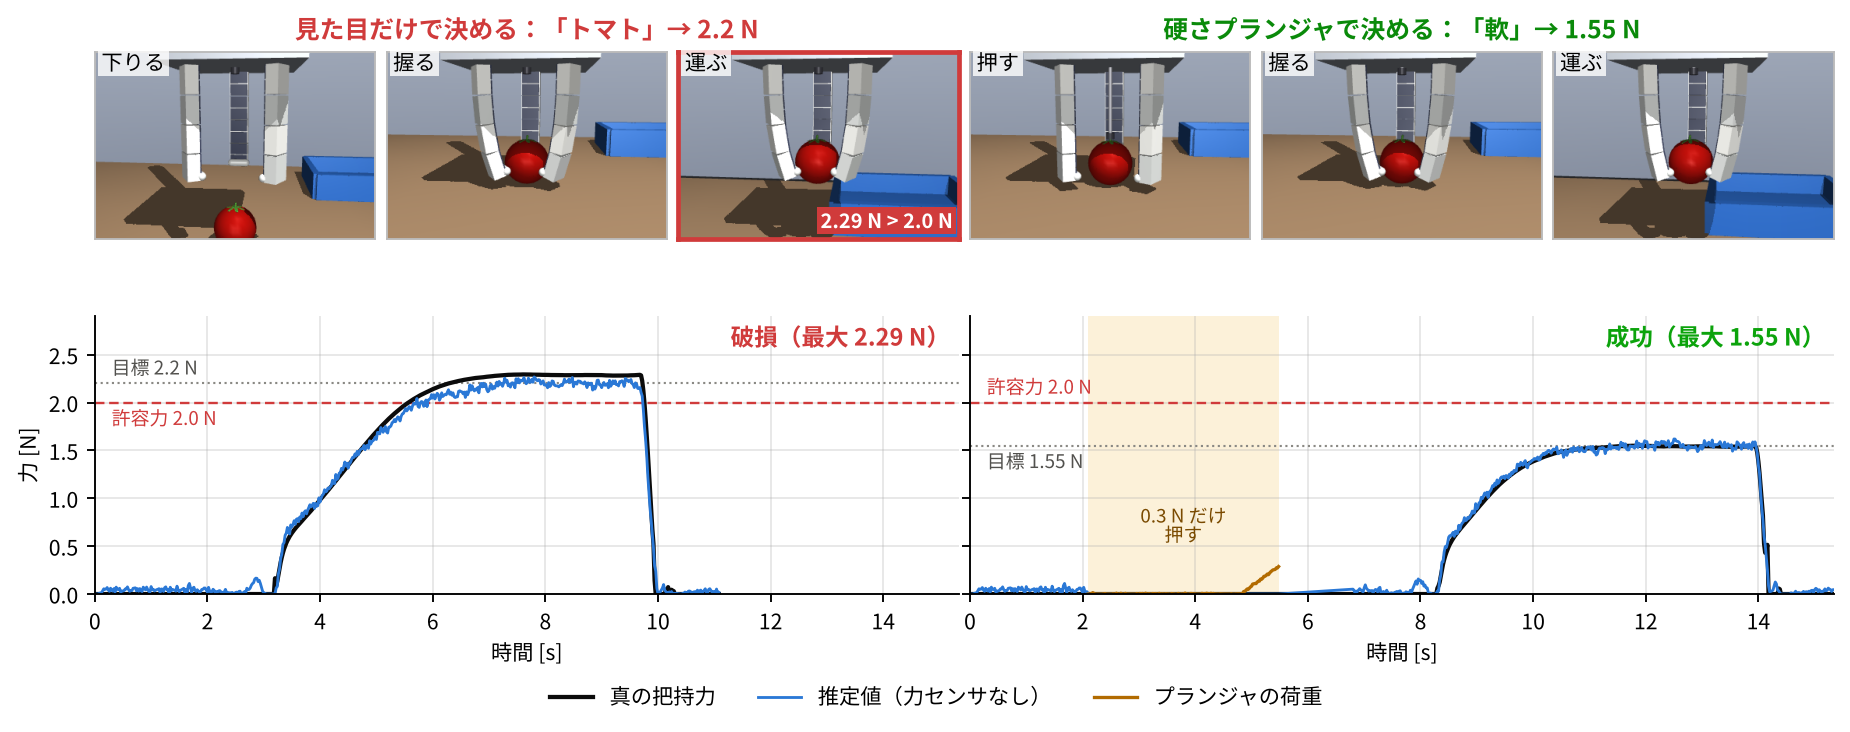
\includegraphics[width=0.97\textwidth]{teaser.png}}
{\captionof{figure}{\textbf{本研究の問題と結果．}見た目は普通の中玉トマトだが，中身は過熟（許容力 2.0\,N）．
左：見た目から「トマト＝2.2\,N」で握ると，真の把持力（黒）が許容力（赤破線）を超えて潰れる．
右：先に硬さプランジャで 0.3\,N だけ押して「軟」と判定し，1.55\,N で握ってトレーへ置く．
青は力センサを使わない推定値，橙はプランジャの荷重である．最大値は 60\,ms の移動平均（破損の判定と同じ）．画像はシミュレーション（MuJoCo）で，へたや指の色は描画だけのもの（質量も接触もなく，接触の計算は球と楕円体のまま）．}
\label{fig:teaser}}
\end{center}
\vspace{2mm}
]

\section{はじめに}
\textbf{背景．}飲食料品製造業では令和 10 年度に就業者が約 21 万人不足すると見込まれている\cite{moj2024}．
食品工場の自動化で最後まで人手が残るのは，形と硬さがばらつく食材を傷めずに扱う工程である\cite{nikkei2025}．
硬さは画像に映らない隠れ状態である．実際の過熟果は色が変わることもあるが，本研究は見た目を完全に同じにした最悪の場合を扱う．このとき，画像からの識別は原理的に不可能である．
本研究でいう力センサは，把持力を校正済みの値として直接測るセンサ（指先のロードセルなど）を指す．布状スキンは接触の位置を知るために使い，その出力を力の値としては使わない．

\textbf{問い．}力センサを持たない柔らかい指を前提に，次の 3 問を立てた．
\begin{description}[leftmargin=0em,labelindent=0em,itemsep=0.5mm]
\item[Q1] 力センサなしで（内圧・曲げ・スキンの接触位置から）把持力を推定し，潰さず落とさない力で握れるか．
\item[Q2] 見た目が同じで硬さだけが違う物体を，把持の前に見分けられるか．指で触るだけで足りるか．
\item[Q3] 人手のラベル付けなしで，判断の学習に使えるデータを作れるか．
\end{description}
あわせて，物理パラメータの根拠（\ref{sec:twin} 節），物理エンジンを替えたときの再現性（\ref{sec:sim2sim} 節），人工筋肉と指のモデル誤差への頑健性（\ref{sec:robust} 節），物体の大きさが変わったときのふるまい（\ref{sec:size} 節）を確かめた．

\textbf{貢献．}
\begin{enumerate}
\item \textbf{MuJoCo と PhysX で共有する制御コア．}物体の個体・人工筋肉・センサ・推定器・制御器・成否の判定を共通の制御コア（\texttt{twin\_core.py}）に置き，物理エンジンには指と物体の動力学だけを任せた．接触剛性は両エンジンで同じ手順で測り，文献値（N/mm）に合わせた．
\item \textbf{触覚で作用点を求める固有感覚推定．}指の曲げ不足から力を求めるには，力がどこに掛かるかが要る．布状スキンの出力で重み付けたてこの和でこれを与え，推定誤差を \V{q1.tip.mae}\,N から \V{q1.learned.mae}\,N に下げた．
\item \textbf{判別マップから決めたセンサ構成．}剛性比とセンサ雑音を掃引し，指で触るだけでは，想定した雑音で剛性比 2.5 の判別正解率がトマト \V{pm.tomato.finger}\,\%・いちご \V{pm.strawberry.finger}\,\% にとどまることを示した．このマップから，把持の前に押す硬さプランジャを加えた．
\item \textbf{比較対象と失敗の内訳．}比較対象は，区分ごとに調整した内圧表（開ループ），「弱く握り始めて滑ったら強める」方策，正解の区分を与える上限である．内圧表が閉ループに劣らない条件と劣る条件（物体の大きさ）を分けて示し，失敗の型と信頼区間も示した．
\end{enumerate}

\textbf{要求．}用途から数値の要求を先に置き，結果と照らした（表\ref{tab:req}）．
\begin{table}[t]
\centering\small
\caption{要求と達成状況．[ ] は Wilson 95\,\% 信頼区間~\cite{wilson1927}（\%）．R3・R5・R8 は点推定，R4・R6 は区間の上端で判定した．R1 は学習に使っていない軌道，R2 は接触中の平均絶対誤差，R7 は画像＋プランジャの 5 分割交差検証の平均，R8 は空中較正（\ref{sec:robust} 節）ありの値（$n=50$）．}
\label{tab:req}
\footnotesize
\setlength{\tabcolsep}{3pt}
\begin{tabular}{@{}L{40mm}rl@{}}
\toprule
要求 & 目標 & 結果 \\
\midrule
R1 筋肉モデルの曲げ RMSE & $\le$3° & \V{req.R1} \\
R2 力推定の誤差（MAE） & $\le$0.2\,N & \V{req.R2} \\
R3 基本 5 物体の成功率 & $\ge$90\,\% & \V{req.R3} \\
R4 基本 5 物体の破損率 & $\le$5\,\% & \V{req.R4} \\
R5 見た目が同じ物体の成功率 & $\ge$85\,\% & \V{req.R5} \\
R6 全 7 物体の破損率 & $\le$5\,\% & \V{req.R6} \\
R7 区分の正解率 & $\ge$95\,\% & \V{req.R7} \\
R8 筋肉が $\pm$20\,\% ずれたときの成功率 & $\ge$90\,\% & \V{req.R8} \\
\bottomrule
\end{tabular}
\end{table}

\section{関連研究}
\textbf{ロボット基盤モデルと触覚．}$\pi_0$~\cite{black2024pi0} や GR00T N1~\cite{nvidia2025gr00t} の入力は主に画像・言語・関節状態である．触覚の重要性は指摘されているが，データの不足が課題とされる~\cite{kawaharazuka2025}．本研究は，触覚付きのデータをシミュレーションで量産する側から取り組む．

\textbf{触覚による把持と物体の識別．}Romano ら~\cite{romano2011} は触覚から接触・保持・滑りの段階を判定し，把持力を調整した．Spiers ら~\cite{spiers2016} は 1 回の把持から物体を識別した．Scimeca ら~\cite{scimeca2019} は多点の押し込みで果実の熟度を推定した．本研究は「指で触るだけで足りるか」を，剛性比とセンサ雑音の判別マップとして定量化した点が異なる．
青果の硬さは，ペネトロメータで押し込んで測るのが標準的な方法である（Magness--Taylor 法~\cite{magness1925}．果肉を貫く破壊試験）．本研究は 0.3\,N で止める非破壊の押し込みで，指による測定が足りない範囲をマップで示し，それに基づいて測定器をグリッパに組み込んだ．

\textbf{センサなしの力推定．}Shuto と Vargas~\cite{shuto2026} は，モータ電流から推定した力と剛性の下限で，ひずみに上限を設けた．本研究は柔らかい指のたわみから力を推定し，作用点を触覚で補う．

\textbf{アクチュエータの学習モデル．}Hwangbo ら\cite{hwangbo2019} はアクチュエータをネットワークで同定した．Thuruthel ら\cite{thuruthel2019} はソフトアクチュエータの状態を再帰ネットワークで推定した．本研究は，学習モデルと物理の形を持つ小さなモデルを同じ条件で比べる．

\textbf{物性を推定して動作を変える．}GenDOM~\cite{kuroki2024gendom} は柔軟物の物性パラメータを推定し，方策を条件付けた．本研究は，把持の前に押し込んで物性を直接測る．

\begin{figure*}[t]
\centering
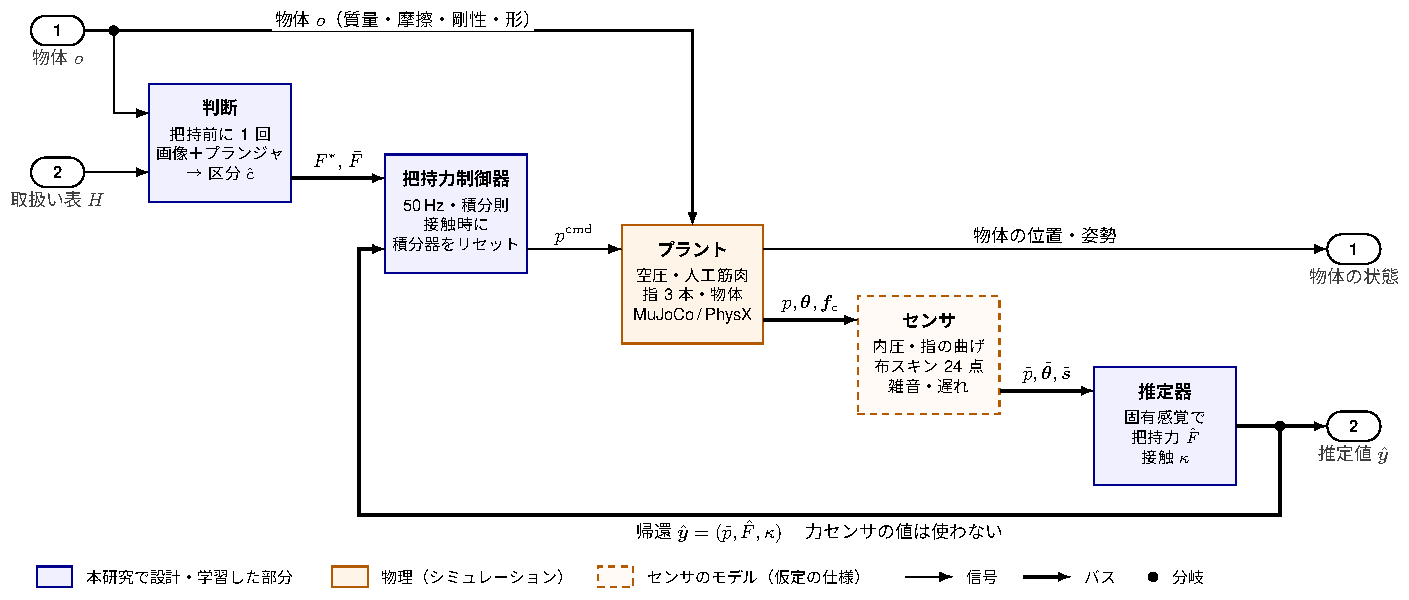
\includegraphics[width=\textwidth]{fig_block_top.pdf}
\caption{\textbf{システムの構成（最上位）．}力センサの値は帰還しない．制御器に戻るのは推定値の束 $\hat{\bm y}=(\tilde p,\hat F,\kappa)$ だけである（$\kappa$ は接触フラグ，式 (4)）．$p,\bm\theta,\bm f_c$ はプラントの真の内圧・関節角・接触力で，$\bm f_c$ はスキンのモデルの入力と，成否の判定・データの記録にだけ使い，制御器には帰還しない．ガントリの動き（接近→下降→把持→持ち上げ→搬送→載置）は状態機械で，図では省いた．各ブロックの中身は図\ref{fig:blockdetail}．}
\label{fig:blocktop}
\end{figure*}

\begin{figure*}[t]
\centering
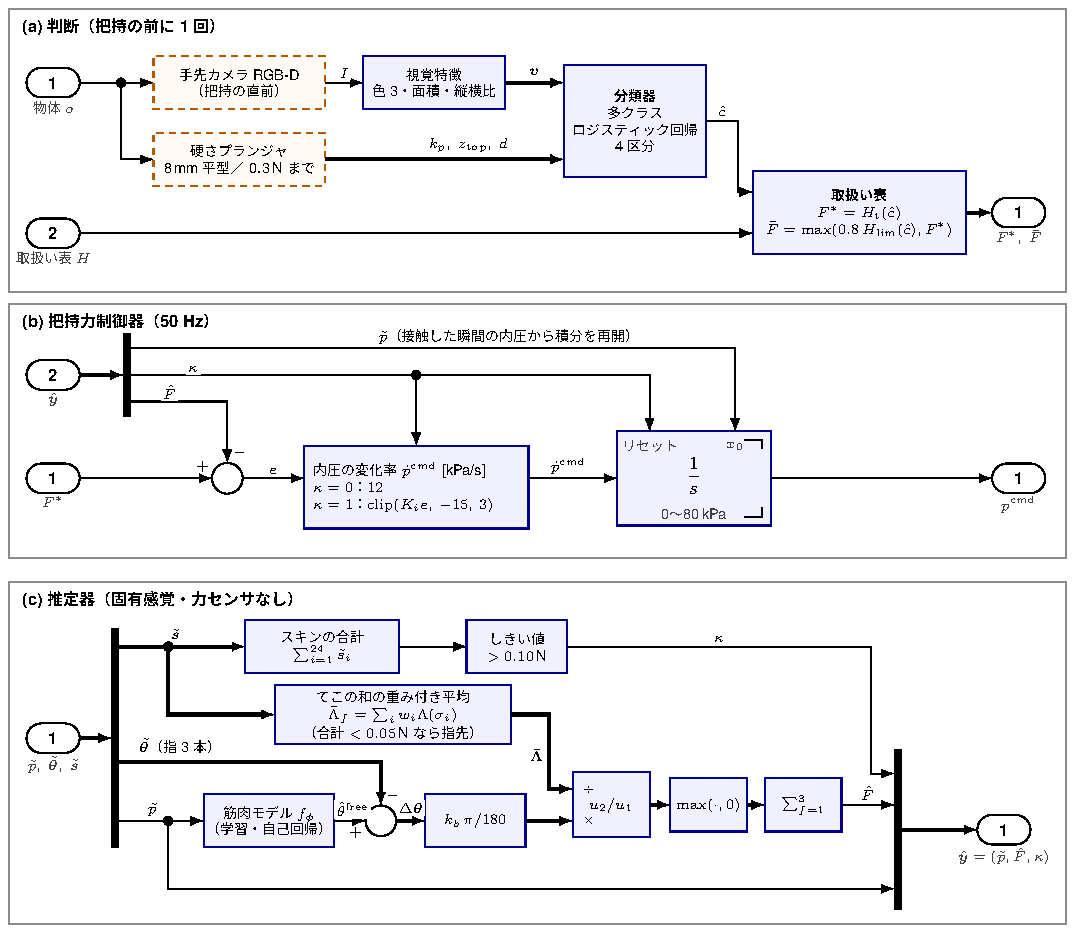
\includegraphics[width=0.94\textwidth]{fig_block_detail.pdf}
\caption{\textbf{サブシステムの中身．}(a) 判断：画像の特徴とプランジャの測定から取扱い区分 $\hat c$ を決め，取扱い表から目標把持力 $F^*$ と再把持の上限 $\bar F$ を引く．$k_p$ は荷重と変位の傾き，$z_{\mathrm{top}}$ は上面の高さ，$d$ は 0.3\,N に達するまでの押し込み量．
(b) 把持力制御器：接触前は 12\,kPa/s で閉じ，接触した瞬間に積分器を測定内圧 $\tilde p$ から再開する．以後は力の誤差 $e$ の積分則で，増圧側を 3\,kPa/s に制限する．$\bar F$ は再把持の状態機械（\ref{sec:decide} 節）が使い，(b) は $F^*$ だけを使う．
(c) 推定器：筋肉モデルの自由曲げ $\hat\theta^{\mathrm{free}}$ と実測の曲げの差を，スキンの出力で重み付けたてこの和 $\bar\Lambda$ で割って力にする（式\eqref{eq:force}，$w_i$ はスキン各点の出力の割合）．スキンの合計が 0.05\,N 未満の指は，作用点を指先とする．$k_b\pi/180$ は曲げ剛性 [N\,m/rad] と度からラジアンへの換算．
枠の色と線の意味は図\ref{fig:blocktop}と同じで，太線は複数の信号の束（バス）である．}
\label{fig:blockdetail}
\end{figure*}

\section{システム}
制御スタックを周期の違う層に分けた（表\ref{tab:stack}，図\ref{fig:blocktop}）．
判断は把持ごとに 1 回で，把持力の閉ループは 50\,Hz で回る．
実機では M5Stack（ESP32）がポンプと電磁弁で内圧を作り，内圧と曲げを配信する設計とした．このグリッパの実機は未製作である．
制御器は ROS~2 のアクション（\texttt{GripperCommand}）として実装し，rclpy のスタブで動作を確かめた．

\begin{table}[t]
\centering\small
\caption{制御スタックの層と周期}
\label{tab:stack}
\begin{tabular}{@{}L{22mm}L{13mm}L{40mm}@{}}
\toprule
層 & 周期 & 役割 \\
\midrule
判断 & 把持ごと & $\hat c\to F^*,\ \bar F$ \\
硬さプランジャ & 把持ごと & 0.3\,N まで押し，傾き $k_p$ を測る \\
力の閉ループ & 50\,Hz & $\hat F\to F^*$ になる内圧指令 \\
空圧供給 & 連続 & 内圧の追従（時定数 0.25\,s） \\
物理エンジン & 1\,kHz & 指と物体の接触 \\
\bottomrule
\end{tabular}
\end{table}

\section{デジタルツインの物理}
\label{sec:twin}
\subsection{セル，指，物体}
指はシリコーン製の空圧人工筋肉（PneuNets 型~\cite{mosadegh2014}）を想定した．3 本を 120° 間隔に置き，各指を長さ $L=26$\,mm の剛体リンク 4 個と回転関節で近似した（擬似剛体モデル~\cite{howell2001}）．
関節は剛性 $k_b=0.5$\,N\,m/rad の位置サーボで，目標角は自由曲げの $1/4$ ずつとした．接触があると関節が目標から遅れ，指は受動的に物体に倣う．
物体の寸法・質量・接触剛性は文献から決め，許容力は卵以外は仮定した（表\ref{tab:obj}，根拠は \texttt{docs/physical\_parameters.md}）．
トマトの硬さは熟度によって緑熟 3.58，ピンク 1.74，レッド 1.16\,N/mm と下がる~\cite{vursavus2017}．これに合わせて，熟した中玉トマトを 1.5\,N/mm とした．文献の値は直径 4\,mm の平型プローブで測ったもので，これを指の接触の剛性としてそのまま使った（仮定）．
過熟の 2 物体は，見た目を同じにしたまま，剛性を 1/2.5 にし，許容力を下げた．比の 2.5 は，熟度段階のあいだの比（ライトレッドとレッドで 1.3 倍，緑熟とレッドで 3.1 倍）の範囲にある．比そのものへの依存は\ref{sec:probe}節の判別マップで調べた．
把持力 $F$ は 3 指の法線力の和 $F=\sum_f F_f$ とし，許容力もこの和で定義した．破損は本来 1 接触あたりの圧力で決まるので，これは 3 指がほぼ均等に押す場合の近似である．卵の赤道方向の破断力は板圧縮で 38〜45\,N~\cite{krivanek2016} で，1 接触あたりの値なので和とは直接比べられないが，和で 25\,N（1 指あたり約 8\,N）は十分に安全側である．
各試行で，質量 $\pm$15\,\%，摩擦 $\pm$20\,\%，接触剛性 $\pm$20\,\%（いずれも一様分布），置き場所，向きを乱数で振る．こうして生成した物体の実体を「個体」と呼ぶ．
乱数の種は $[\text{試行番号},\ \mathrm{crc32}(\text{物体名})]$ で，同じ試行番号なら MuJoCo と PhysX は同じ個体を扱う．

\begin{table}[t]
\centering\small
\caption{評価物体．剛性は指 1 本との接触の値，許容力は 3 指の法線力の和．$H_{\mathrm t}$・$H_{\mathrm{lim}}$ は取扱い表の区分ごとの目標と許容力．$^\dagger$見た目は上の物体と同じ．}
\label{tab:obj}
\setlength{\tabcolsep}{3pt}
\begin{tabular}{@{}lrrrlrr@{}}
\toprule
物体 & 質量 & 剛性 & 許容力 & 区分 & $H_{\mathrm t}$ & $H_{\mathrm{lim}}$ \\
 & [g] & [N/mm] & [N] & & [N] & [N] \\
\midrule
いちご & 20 & 1.0 & 3.0 & 脆 & 2.2 & 3.0 \\
卵 & 56 & 剛 & 25 & 頑丈 & 3.0 & 25 \\
木綿豆腐 & 36 & 0.5 & 4.0 & 脆 & 2.2 & 3.0 \\
中玉トマト & 43 & 1.5 & 5.0 & 脆 & 2.2 & 3.0 \\
ボルト（M12） & 35 & 剛 & -- & 頑丈 & 3.0 & 25 \\
\midrule
過熟中玉トマト$^\dagger$ & 43 & 0.6 & 2.0 & 軟 & 1.55 & 2.0 \\
過熟いちご$^\dagger$ & 20 & 0.4 & 1.5 & 極脆 & 1.2 & 1.5 \\
\bottomrule
\end{tabular}
\end{table}

\subsection{接触剛性をエンジンに入れる}
文献値は N/mm で与えられる．しかし MuJoCo は接触を時定数 $t_c$ で指定するので，そのままでは入れられない．
solimp と減衰比を一定にすると，準静的な接触は線形ばねとしてふるまい，その剛性は $K\propto m_{\mathrm{eff}}/t_c^2$ となる~\cite{todorov2012}．比例定数を決める実効質量 $m_{\mathrm{eff}}$ は，測定から同定した（数値上の定数で，指の質量そのものではない）．
手順は次の通りである．理想的な力ループで 1\,N で握り，指 1 本ごとに「力 ÷ めり込み」を測る．目標との比の平方根で $t_c$ を補正し，これを繰り返す（$t_c$ が積分刻みの数倍まで短くなると比例が崩れるため，2〜3 回の反復を要した）．
補正後は，剛性を数値で与えた 5 物体すべてで測定剛性が目標の \V{cal.mj.maxdev} 以内に入った．
PhysX は「コンプライアント接触」に剛性を N/m で直接与えられる．ただし剛性は接触点ごとに掛かるので，同じ手順で測って確かめた（目標との比 \V{cal.px.range}）．

\subsection{センサ}
センサは実在の部品を想定した仮定のモデルである．
\begin{itemize}
\item 内圧：雑音 0.2\,kPa．
\item 指の曲げ：雑音 0.3°，分解能 0.1°，時定数 $\tau_s=20$\,ms．
\item 布状の触覚スキン（以下，スキン．1 節に 2 点，指 1 本に 8 点，計 24 点）：不感帯 0.08\,N，雑音 0.02\,N，感度のばらつき 10\,\%，隣への漏れ 10\,\%，時定数 30\,ms，12\,bit．
\item 硬さプランジャ：ロードセル雑音 5\,mN，エンコーダ雑音 2\,µm．
\end{itemize}

\section{手法}
\subsection{筋肉モデル}
空圧の人工筋肉は，内圧 $p$ に対して不感帯・飽和・遅れ・履歴を持つ（図\ref{fig:act}a）．
評価には，この形を持つ「模擬筋肉」を真のプラントとして使った（不感帯 6\,kPa，飽和曲線，曲げの遅れの時定数 0.12\,s，履歴の幅 6°）．履歴は上昇と下降の枝のあいだを動く遊び要素で表し，内圧が少し戻っただけでは曲げは変わらない．
自由曲げ $\theta^{\mathrm{free}}$ のモデルは次の 5 つを比べた．
\begin{itemize}
\item \textbf{直線}：$\beta p$．同定データへの最小二乗．
\item \textbf{静特性の表}：不感帯と飽和曲線だけを持ち，遅れはない．
\item \textbf{グレーボックス}：5 パラメータで，不感帯＋飽和＋1 次遅れ．履歴は持たない（ステップ試験から技術者が書く形）．
\item \textbf{グレーボックス＋遊び}：上に幅 $w$ の遊び要素を加えた 6 パラメータ．模擬筋肉そのものが同じ要素で作られているので，このモデルは構造を最初から知っている（実機ではこの保証はない）．
\item \textbf{学習モデル}：MLP $[\tilde p_k, \dot{\tilde p}_k, \hat\theta_{k-1}]\to\hat\theta_k$．隠れ層 $48\times 2$，自己回帰で使う．内圧の雑音で偏らないよう，入力は時定数 40\,ms で前処理した．
\end{itemize}
同定データは段差・ランプ・正弦と，把持に似た内圧（速い増圧，接触後を模した 1〜5\,kPa/s の増圧，小さな修正を含む保持，排気）の 100 軌道で，内圧と曲げには測定の雑音を加えた．
学習に使っていない 20 軌道での RMSE は，直線 \V{act.linear}°，静特性の表 \V{act.static}°，グレーボックス \V{act.greybox}°，グレーボックス＋遊び \V{act.gbplay}°，学習モデル \V{act.learned}° だった．把持に使う内圧域に限ると，グレーボックス \V{act.greybox.grip}°，グレーボックス＋遊び \V{act.gbplay.grip}°，学習モデル \V{act.learned.grip}° である（同定された遊びの幅は 4.9°，真値は 6°）．この RMSE は速い変化も含む軌道全体の値で，把持中の偏りとは別に見る必要がある（\ref{sec:q1} 節）．
直線モデルは，把持に使う \V{rec.lo}〜\V{rec.hi}\,kPa で自由曲げを過小に見積もる（図\ref{fig:act}a）．

\begin{figure*}[t]
\centering
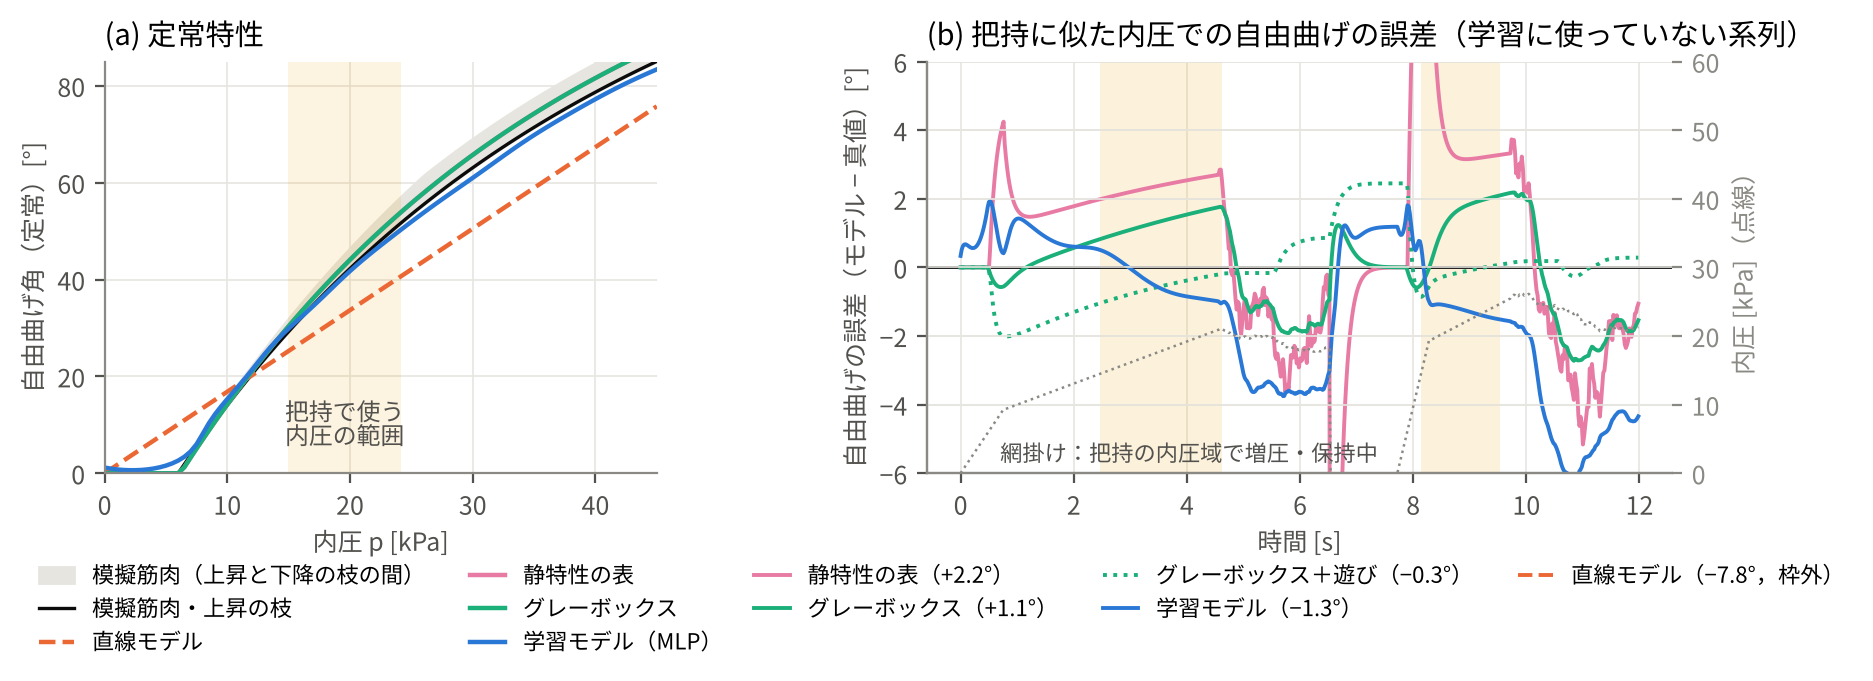
\includegraphics[width=0.9\textwidth]{fig_actuator.png}
\caption{\textbf{筋肉のモデル．}(a) 定常特性．灰色の帯は模擬筋肉の履歴（上昇と下降），黄色は把持で使う内圧の範囲．直線モデルは，この範囲で自由曲げを 3〜13°（上昇と下降の中線に対して）小さく見積もる．
(b) 学習に使っていない，把持に似た内圧の系列での自由曲げの誤差（モデル − 真値）．(a) では見やすさのため遊びつきのグレーボックスを省いた．凡例の数字は，30 系列（RMSE の 20 軌道とは別）で把持の内圧域を増圧・保持しているあいだの誤差の中央値である．誤差が正だと，力を大きく見積もって弱く握る．}
\label{fig:act}
\end{figure*}

\subsection{固有感覚による把持力の推定}
\label{sec:est}
指 $f$ の付け根から指に沿って距離 $\xi$ の点に，指に垂直な力 $F_f$ が掛かるとする．関節 $j$（位置 $\xi_j=jL$）は腕の長さ $(\xi-\xi_j)^+$ のトルクを受け，角度 $F_f(\xi-\xi_j)^+/k_b$ だけ戻される．
角度はすべてラジアンで扱う（センサの値は度で，図\ref{fig:blockdetail}(c) の $k_b\pi/180$ で換算する）．
指 1 本の曲げ不足 $\Delta\theta_f=\hat\theta^{\mathrm{free}}-\tilde\theta_f$ は各関節の戻りの和なので，
\begin{equation}
\Delta\theta_f=\frac{F_f\,\Lambda(\xi)}{k_b},\qquad \Lambda(\xi)=\sum_{j=0}^{3}(\xi-\xi_j)^+ .
\end{equation}
$\Lambda$ を「てこの和」（各関節から作用点までの腕の長さの和，長さの次元）と呼ぶ．式は指がまっすぐなときの腕の長さで書いており，指が曲がると，関節より先のリンクの腕はそれぞれ累積角の余弦倍に縮む（誤差は $O(\phi^2)$ で，把持中の関節角 $\phi\approx10°$ では $\Lambda$ が約 3\,\% 小さくなる）．
これを逆に解き，3 本の和を把持力の推定とする．
\begin{equation}
\hat F=\sum_{f=1}^{3}\max\!\Bigl(\frac{k_b\,\Delta\theta_f}{\bar\Lambda_f},\,0\Bigr),\qquad
\bar\Lambda_f=\frac{\sum_i \tilde s_{f,i}\,\Lambda(\sigma_i)}{\sum_i \tilde s_{f,i}}
\label{eq:force}
\end{equation}
$\bar\Lambda_f$ は，その指のスキン 8 点の出力 $\tilde s_{f,i}$ で重み付けた，各点の位置 $\sigma_i\in\{0.25L,0.75L,\dots,3.75L\}$ でのてこの和の平均である．いくつかの点で触れると曲げ不足は各点の寄与の和になるので，重心の $\Lambda$ ではなく $\Lambda$ の重み付き平均を使う（$\Lambda$ は下に凸なので，重心の $\Lambda$ では力を大きく見積もる）．スキンの合計が 0.05\,N 未満のときは，指先（$\Lambda=10L=0.26$\,m）と仮定する．
作用点を指先に固定すると，接触が指先より根元側にあるとき $\Lambda$ を過大に見積もる．その結果，力を $\Lambda(\xi)/\Lambda(4L)$ 倍（$\xi$ は真の作用点）に過小評価し，制御器はその分だけ強く握る．
式\eqref{eq:force} の対数をとって微分すると，推定の相対誤差は 3 つの項に分かれる（$\delta x$ は量 $x$ のモデルの値から真値を引いた差）．
\begin{equation}
\frac{\delta\hat F_f}{F_f}\;\simeq\;\frac{\delta k_b}{k_b}\;+\;\frac{\delta\hat\theta^{\mathrm{free}}-\delta\tilde\theta_f}{\Delta\theta_f}\;-\;\frac{\delta\bar\Lambda_f}{\bar\Lambda_f}
\label{eq:errsplit}
\end{equation}
第 1 項は曲げ剛性の誤差で，そのまま比例して入る（\ref{sec:robust} 節）．第 2 項は筋肉モデルの自由曲げの偏りで，分母の曲げ不足は目標 2.2\,N のとき指 1 本あたり約 20° なので，1° の偏りが力の約 5\,\% になる．曲げ不足は力に比例するので，この項は $1/F^*$ に比例して大きくなる．目標 1.2\,N の極脆では 1° が約 9\,\% にあたり，許容力までの余裕が最も小さい物体で推定誤差が最も大きくなる．第 3 項は作用点の誤差である．指先の丸みでの接触は，スキンの最も先の点（$3.75L$）より先の約 $3.87L$（把持中の接触点の中央値）にあり，$\Lambda(3.87L)/\Lambda(3.75L)=9.48/9.0$ から，$\bar\Lambda$ を約 5\,\% 小さく見積もって力を約 5\,\% 大きく見積もる．
このほか，垂直でない力の成分と曲げセンサの遅れ（増圧中は $\tau_s\dot\theta$ だけ遅れる）が残る．各項の実測は\ref{sec:q1}節に示す．

\subsection{把持力の制御}
制御則は図\ref{fig:blockdetail}(b) の通りで，式で書くと次のようになる．
\begin{equation}
\dot p^{\mathrm{cmd}}=\begin{cases}12 & (\kappa=0)\\ \mathrm{clip}\bigl(K_i(F^*-\hat F),\,-15,\,3\bigr) & (\kappa=1)\end{cases}\ \ [\mathrm{kPa/s}]
\end{equation}
ここで $K_i=4$\,kPa/(N\,s) である．接触フラグ $\kappa$ はスキンの合計が 0.10\,N を超えたことで立て，その時刻 $t_\kappa$ に積分器を測定内圧から再開する（$p^{\mathrm{cmd}}(t_\kappa^+)=\tilde p(t_\kappa)$）．再開しないと，供給系の遅れの分だけ行き過ぎる．
接触後の内圧から力への静的な傾きは $\partial F/\partial p\approx\V{ctl.dFdp}$\,N/kPa だった（5 物体の平均）．
目標近傍の小信号で線形化すると閉ループは 1 次系になり，時定数は $\tau_{\mathrm{cl}}=1/(K_i\,\partial F/\partial p)\approx\V{ctl.taucl}$\,s である．交差周波数は約 1\,rad/s で，ここでの位相遅れは供給系（時定数 0.25\,s）14°，筋肉の遅れ（0.12\,s）7°，曲げセンサ（20\,ms）と 1 サンプルの遅れ 2° の計約 23° なので，位相余裕は約 67° ある（増圧の制限と履歴の遊びを除いた線形化での値）．
実際の立ち上がりは，増圧側の制限 3\,kPa/s で決まる．力の増加はおよそ $3\,\partial F/\partial p\approx0.75$\,N/s で，目標 2.2\,N の 8 割に届くまで \V{ctl.rise22}\,s かかった（シード 0〜4）．この値から見積もる 2.3\,s より短いのは，接触した時点ですでに 0.1〜0.4\,N（中央値約 0.3\,N）の力が出ているためである．
制限を外すと速くなるが，柔らかい物では力がオーバーシュートする．本研究は潰さないことを優先した．

\subsection{握る高さ}
丸い物は，赤道より下を深く握るほど重さを支えやすい．しかし深すぎると，把持力の上向きの成分で上へ押し出される．
赤道から下向きに測った指先の接触角を $\alpha$ とする．法線力の和 $F^*$ の上向き成分は $F^*\sin\alpha$，摩擦で抑えられる上限は $\mu F^*\cos\alpha$ なので，$F^*(\sin\alpha-\mu\cos\alpha)>mg$ のとき物体は押し出される．
そこで「$F^*(\sin\alpha-0.8\mu\cos\alpha)\le 0.5\,mg$」，すなわち上向きの正味の力を重量の半分以下に抑える最も深い $\alpha$ を選んだ（探索範囲は $\sin\alpha\le0.6$）．$0.8\mu$ は摩擦の乱数の下端である．公称の $\mu$ と質量 $m$ は，見た目から推した物体のものを使う．
$\alpha$ に対応する手の高さは，指先の運動学から求める．楕円体（いちご・卵）では $\alpha$ を楕円のパラメータ角で近似したので，実際の法線の傾きはこれより数度大きい．箱と円柱は，高さの半分を握る．

\subsection{硬さの測り方：指か，プランジャか}
\label{sec:probe}
最初の設計では，0.8\,N まで弱く握ったときの「スキンの力の増分 ÷ 追加の曲げ」で硬さを測った（指プローブ）．
しかし指は果実よりはるかに柔らかい．指先のコンプライアンスは $\Sigma_j l_j^2/k_b=0.041$\,m/N（$l_j=4L-\xi_j$ は関節 $j$ から指先までの距離）で，果実（1/1500〜1/400\,m/N）の 16〜61 倍ある．そのため，果実の変形は指自身のたわみに埋もれる．
そこで，過熟の剛性比（1〜4）と曲げセンサの雑音（0〜1°）を掃引した．各点 30 個体で 1 次元のしきい値を 5 分割交差検証し，判別マップを作った（図\ref{fig:map}）．
想定の雑音 0.3° では，比 2.5 で正解率はトマト \V{pm.tomato.finger}\,\%，いちご \V{pm.strawberry.finger}\,\% にとどまる．雑音がなくても \V{pm.tomato.finger0}\,\% と \V{pm.strawberry.finger0}\,\% で，個体差（質量・摩擦・姿勢）の影響が残る．
これを受けて，掌の中心に直径 8\,mm の平型プランジャを置いた．把持の前に上面を 1\,mm/s で押し，0.3\,N か 3\,mm で止め，荷重と変位の傾き $k_p$ [N/mm] を測る．
先端の接触剛性は，平型圧子の関係 $K=2a_pE^*$（$a_p$ は圧子の半径，$E^*$ は等価弾性率~\cite{sneddon1965,johnson1985}）で，文献の直径 4\,mm の値を 8\,mm に換算して 2 倍とした．
$k_p$ は見かけの剛性で，上面の接触，台側の接触，手（ガントリ）のたわみが直列に入る（$1/k_p=1/k_{\mathrm{top}}+1/k_{\mathrm{bot}}+1/k_{\mathrm{hand}}$）．手のたわみは個体によらないので判別を妨げないが，見かけの剛性比を 1 に近づける．
想定の雑音（2\,µm）では，剛性比 1.5 でトマト \V{pm.tomato.plunger15}\,\%・いちご \V{pm.strawberry.plunger15}\,\%，比 2 以上で \V{pm.tomato.plunger}\,\% だった．雑音が 25 倍（50\,µm）でも，比 2 でトマト \V{pm.tomato.plunger2n50}\,\% を保った．
この値は，個体の剛性のばらつき（一様 $\pm$20\,\%）だけで決まる上限にほぼ一致する（図\ref{fig:map} の太い灰色の線．真の剛性に最適なしきい値を置いたときの正解率で，比 1.25 で 80\,\%，隣り合う熟度段階の比 1.3 で 84.6\,\%，1.5 以上で 100\,\%）．$k_p$ は真の剛性の単調な関数なので，最適なしきい値での上限は手のたわみが直列に入っても変わらない（実験ではクラス平均の中点をしきい値とした）．判別精度を制約するのはセンサ雑音ではなく個体差である．
一方，指プローブは雑音がなくても上限に届かない．指の特徴量（スキンの力に対する曲げの傾き [deg/N]）を指先の変位に換算すると，果実のコンプライアンス（熟したトマトで約 0.7\,mm/N，過熟で約 1.7\,mm/N）のほかに，荷重で曲がる指の形が自由曲げの形からずれる分が入る．後者は指先のコンプライアンス $\Sigma_j l_j^2/k_b=41$\,mm/N に比例し，接触の位置と姿勢で変わる．その変動が 41\,mm/N の 2.4\,\% あれば，熟度の差（約 1.0\,mm/N）と同じ大きさになる（オーダーの見積もり）．

\begin{figure*}[t]
\centering
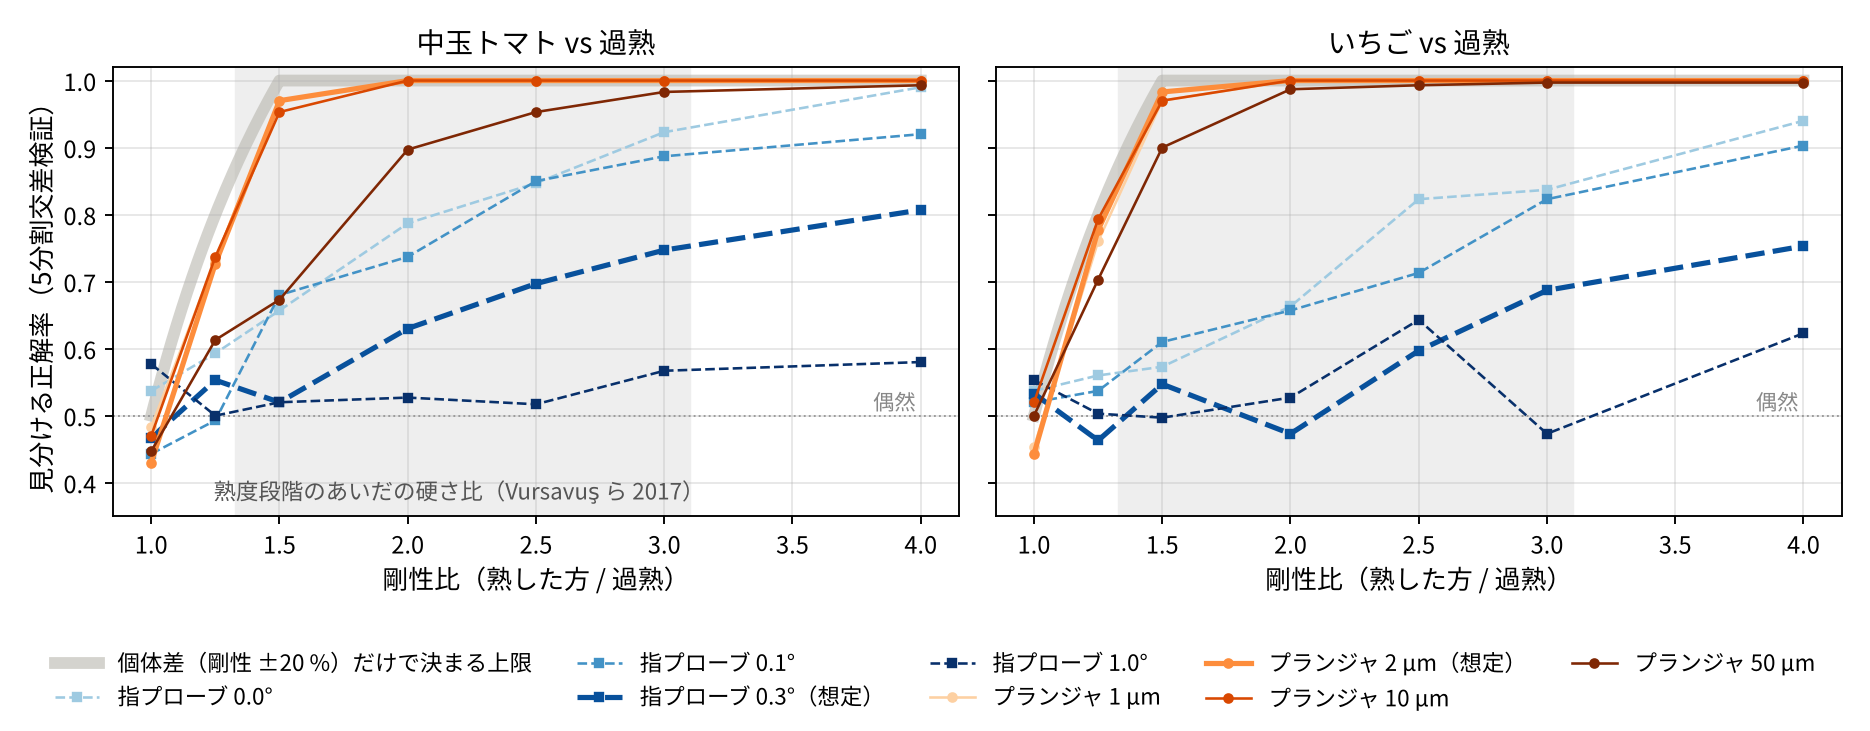
\includegraphics[width=0.92\textwidth]{fig_probe_map.png}
\caption{\textbf{判別マップ．}横軸は熟した方と過熟の剛性比，縦軸は 1 次元のしきい値の 5 分割交差検証の正解率（各点 30 個体，雑音は 5 回の平均）．太い灰色の線は，個体の剛性のばらつき（$\pm$20\,\%）だけで決まる上限．凡例の数字は，指プローブでは曲げセンサの雑音，プランジャでは変位（エンコーダ）の雑音．灰色はトマトの熟度段階のあいだの比~\cite{vursavus2017}．太線が本研究で想定した雑音である．}
\label{fig:map}
\end{figure*}

\subsection{判断と比較対象}
\label{sec:decide}
判断は 4 区分の多クラスロジスティック回帰で行う．入力は画像の特徴 5 個（色 3・面積・縦横比）と，プランジャの $k_p$・上面の高さ・押し込み量である．区分から取扱い表で $F^*=H_{\mathrm t}(\hat c)$ を引く．
把持の前に一度，空中較正（物体のない空中で指を階段状に閉じ，実測とモデルの曲げの差を表にして以後の予測に足す．\ref{sec:robust} 節）で筋肉モデルの偏りを取る．滑ったら $F^*$ を 1.3 倍にして，最大 3 回つかみ直す．再把持で増やす力の上限は $\bar F=\max(0.8H_{\mathrm{lim}}(\hat c),\ F^*)$ とした（つかみ直しで力を下げることはない）．
比較対象は次の通りである．
\begin{itemize}
\item \textbf{内圧表（開ループ）}：区分ごとに，最終内圧を二分探索で調整した表．力の帰還はしない（Q1）．
\item \textbf{見た目だけ}：見た目の区分の $F^*$ を使う．
\item \textbf{弱く握り始める}：全物体を最も弱い区分の目標（1.2\,N）から始め，滑ったら強める．
\item \textbf{指プローブで決める}：指プローブの特徴で分類する．
\item \textbf{力の窓}：区分を使わず，成否ラベルから $P(\text{潰れ}\mid\bm x,F)$ と $P(\text{滑り}\mid\bm x,F)$ を学ぶ．その和を最小にする $F$ を選ぶ．
\item \textbf{正解の区分}：上限として与える．
\end{itemize}

\subsection{自動アノテーション付きデータ}
1 試行ごとに，次のものを同期して書き出す（表\ref{tab:ds}）．
\begin{itemize}
\item 手先カメラの RGB・深度・マスク
\item プランジャの荷重と変位，指プローブ
\item 50\,Hz の内圧・曲げ（実測と真値）・推定把持力と真の把持力・スキン 24 点（出力と真値）
\item 隠れた物理量（質量・摩擦・剛性）と成否
\end{itemize}
目標把持力は 0.5〜4.0\,N から無作為に選ぶ．これで，破損・滑りの事例も十分な数だけ含まれる．
成否は次の通り機械的に決める．
\begin{itemize}
\item 破損：保持中の真の把持力の 60\,ms 移動平均が許容力を超える．
\item 滑り：持ち上げても，物体の中心が台の上面から 8\,cm に届かない（指のあいだから抜ける）．
\item 落下：持ち上げた後，0.1\,s 以上どの指にも触れていない．
\item 成功：持ち上げてトレーに置け，破損がない．
\end{itemize}

\begin{table}[t]
\centering\small
\caption{自動生成したデータ（人手のラベル付けなし，CC BY 4.0）}
\label{tab:ds}
\begin{tabular}{@{}L{12mm}L{60mm}@{}}
\toprule
規模 & \V{ds.n} 試行（7 物体×60），2 CPU で \V{ds.min} 分 \\
時系列 & \V{ds.samples} サンプル（50\,Hz）．$p^{\mathrm{cmd}}$（行動），$\tilde p$，$\hat\theta^{\mathrm{free}}$，$\tilde{\bm\theta}$，$\bm\theta$，$\hat F$，$F$，$\tilde{\bm s}$，$\bm s$ \\
画像 & 手先 RGB・深度・マスク，全体 RGB・マスク \\
ラベル & 物体，見た目，真の区分，隠れた物理量，目標力，成否（\V{ds.outcomes}） \\
品質保証 & 検証器（型・形状・値域・ラベルの整合），ハッシュ，CI．LeRobotDataset v2.1 へ書き出し可 \\
\bottomrule
\end{tabular}
\end{table}

\section{実験と結果}
\begin{figure*}[t]
\centering
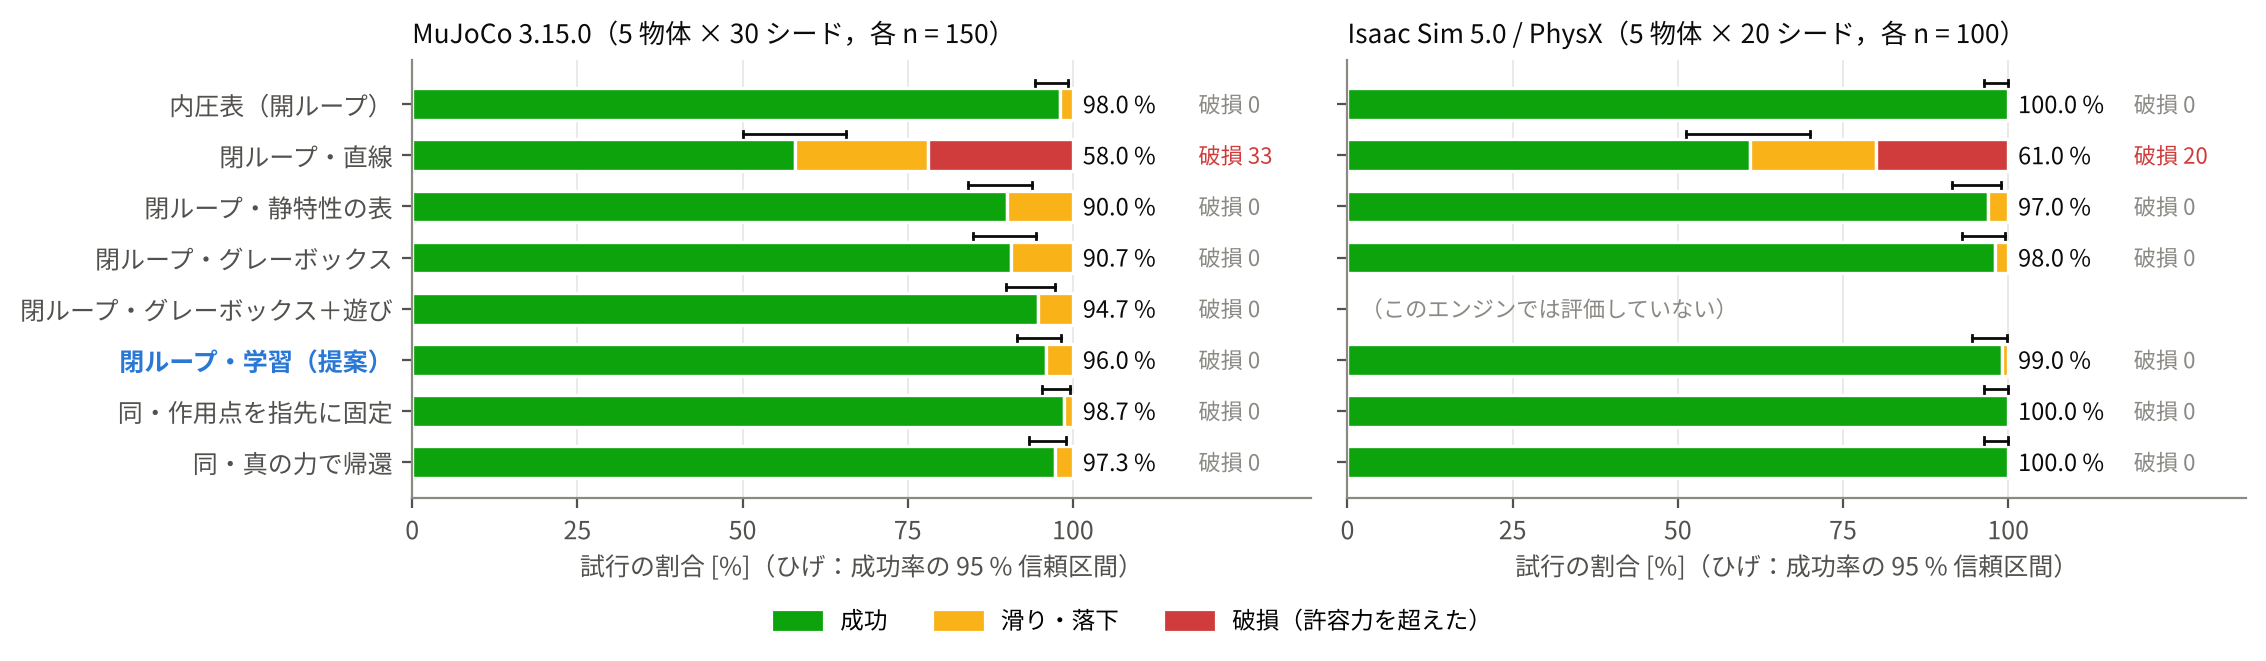
\includegraphics[width=0.98\textwidth]{fig_q1.png}
\caption{\textbf{Q1：把持の結果．}左：MuJoCo．右：Isaac Sim 5.0 / PhysX．ひげは成功率の Wilson 95\,\% 信頼区間．同じ制御コアと同じ物体の個体（同じシード）を，2 つの物理エンジンで走らせた．}
\label{fig:q1}
\end{figure*}

\begin{figure*}[t]
\centering
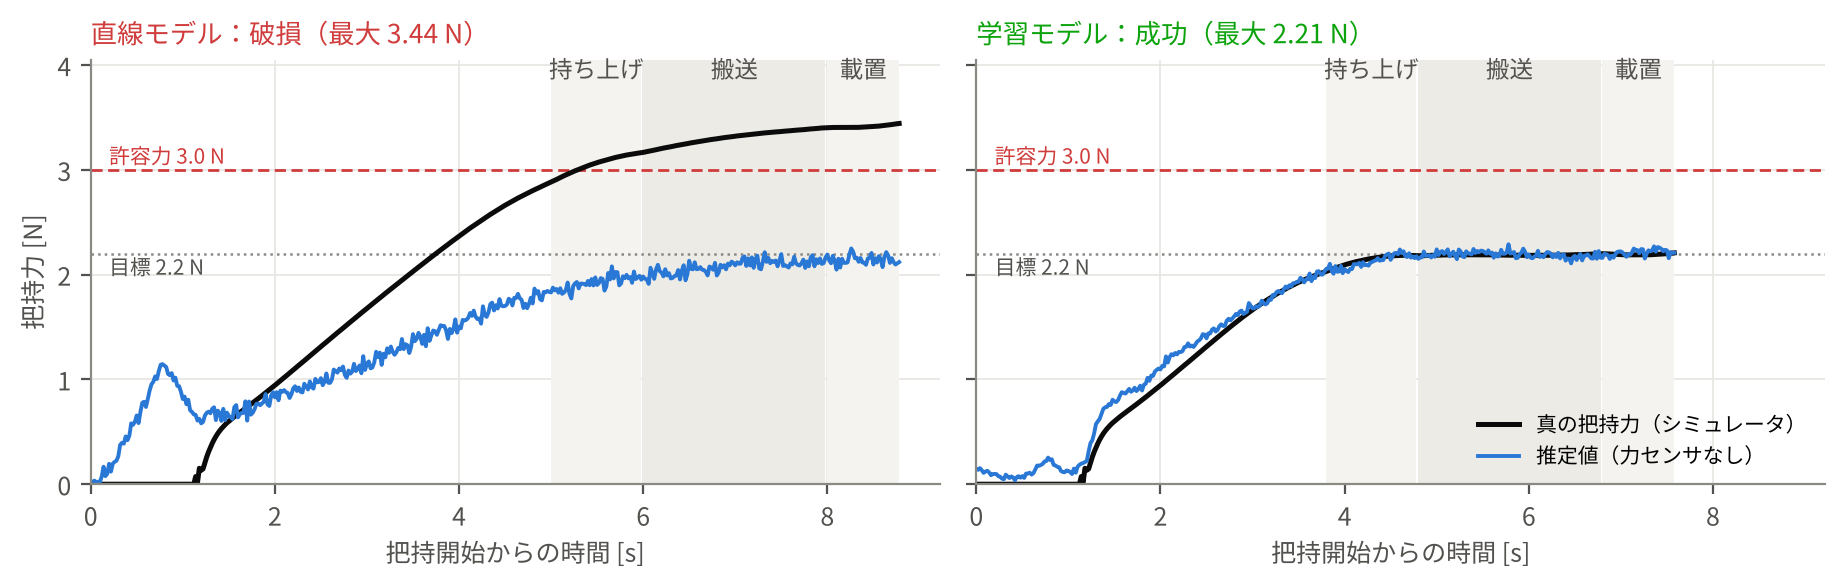
\includegraphics[width=0.9\textwidth]{fig_force_trace.png}
\caption{\textbf{同じいちご・同じシードで，筋肉のモデルだけを替えた．}黒は真の把持力，青は推定値（力センサなし）．直線モデルは力を小さく見積もり続け，制御器が増圧を続けて許容力を超える．搬送中の小さな山は，加減速で物体が指の中で揺れるためである．}
\label{fig:trace}
\end{figure*}

\subsection{条件}
MuJoCo \V{env.mujoco}（時間刻み 1\,ms，制御 50\,Hz）と，Isaac Sim 5.0 の PhysX（1\,kHz，TGS ソルバ）で評価した．
シードは評価 0〜29，データ生成 1000 以降，内圧表の調整 10000 である．接触剛性の合わせ込みにはシード 0〜2 を使った（合わせたのは物体の剛性だけ）．
なお，取扱い表と評価する物体は，開発中に評価シードの結果を見て見直した（剛性の単位の修正，作用点の推定，物体の大きさの変更など）．評価シードは完全に独立な検証ではないので，最終の構成を開発中に一度も使っていないシード \V{ho.seeds} でも走らせた（\ref{sec:holdout} 節）．
Q1 は筋肉モデルそのものを比べるため，空中較正なしで評価した．Q2・大きさ・頑健性（R8）は，配備する手順どおり空中較正ありで評価した．
各方式を同じ（物体，シード）の組で試行した．比較には対応のある McNemar の正確検定~\cite{mcnemar1947} を使い，差の 95\,\% 信頼区間は，対応のある比率の差に対する Newcombe のスコア法（method 10）~\cite{newcombe1998} で求めた（区間は多重比較の補正をしていない）．
事前に決めた \V{t.n} 個の比較に Holm の補正~\cite{holm1979} をかけた（$p_{\mathrm{Holm}}$）．

\subsection{Q1：力センサなしで，潰さず落とさずに握れるか}
\label{sec:q1}
結果を図\ref{fig:q1}と表\ref{tab:q1}に示す．
\begin{table}[t]
\centering\small
\caption{Q1（MuJoCo，5 物体×30 シード，各 $n=\V{q1.n}$）．推定誤差は接触中の平均絶対誤差．}
\label{tab:q1}
\setlength{\tabcolsep}{3pt}
\begin{tabular}{@{}lccc@{}}
\toprule
方式 & 成功 [\%] & 破損 & 推定誤差 [N] \\
\midrule
内圧表（開ループ） & \V{q1.recipe.succ} & \V{q1.recipe.cr} & -- \\
閉ループ・直線 & \V{q1.affine.succ} & \V{q1.affine.cr} & \V{q1.affine.mae} \\
閉ループ・静特性の表 & \V{q1.static.succ} & \V{q1.static.cr} & \V{q1.static.mae} \\
閉ループ・グレーボックス & \V{q1.greybox.succ} & \V{q1.greybox.cr} & \V{q1.greybox.mae} \\
閉ループ・グレーボックス＋遊び & \V{q1.gbplay.succ} & \V{q1.gbplay.cr} & \V{q1.gbplay.mae} \\
\textcolor{prop}{閉ループ・学習（提案）} & \V{q1.learned.succ} & \V{q1.learned.cr} & \V{q1.learned.mae} \\
同・作用点を指先に固定 & \V{q1.tip.succ} & \V{q1.tip.cr} & \V{q1.tip.mae} \\
同・真の力で帰還 & \V{q1.ideal.succ} & \V{q1.ideal.cr} & -- \\
\bottomrule
\end{tabular}
\end{table}
\textbf{直線モデル}は，把持の内圧域で自由曲げを小さく見積もるため，力も小さく見積もり，制御器が増圧を続ける．その結果，いちごを全数（30/30）潰した（図\ref{fig:trace}．ほかに豆腐を 3 件潰した）．
接触前にも推定が 1\,N 前後まで上がる．直線モデルは不感帯（6\,kPa）と遅れを持たないので，空中では実際より大きな曲げを予測し，その差を力と見誤るためである．
ボルトでは逆に，推定値が把持時間（5\,s）内に目標へ届かず，持ち上げ開始時に「物体を失った」判定（$\hat F<0.5F^*$）で中断した．つかみ直しを含めて 4 回試みても \V{q1.affine.bolt.slip}/30 試行で持ち上がらなかった（シード 0 では真の力は約 2.5\,N で，摩擦の上では保持できる値だった）．
不感帯と飽和を持つ 3 つのモデル（静特性の表・グレーボックス・学習）は，どれも破損 0 だった．差は主に豆腐の落下に出た（静特性の表 \V{q1.static.tofudrop} 件，グレーボックス \V{q1.greybox.tofudrop} 件，学習 \V{q1.learned.tofudrop} 件．卵も前の 2 つが \V{q1.static.eggdrop} 件・\V{q1.greybox.eggdrop} 件落とした）．
学習モデルの成功率は \V{q1.learned.succ}\,\%（\V{q1.learned.ci}）で，直線モデルとの差は \V{t.q1.learned-affine.diff}（$p_{\mathrm{Holm}}$ \V{t.q1.learned-affine.p}）である．
グレーボックスとの不一致の組（学習のみ成功：グレーボックスのみ成功）は \V{t.q1.learned-greybox.ab}（$p_{\mathrm{Holm}}$ \V{t.q1.learned-greybox.p}），静特性の表とは \V{t.q1.learned-static.ab}（$p_{\mathrm{Holm}}$ \V{t.q1.learned-static.p}）だった．

落下の差は，推定の偏りから来ている．把持中の推定値÷真値の中央値は，静特性の表 \V{q1.static.bias}，グレーボックス \V{q1.greybox.bias}，学習モデル \V{q1.learned.bias} で，前の 2 つは力を 1 割以上大きく見積もってその分弱く握り（搬送中の真の力÷目標：\V{q1.static.hold}，\V{q1.greybox.hold}，\V{q1.learned.hold}），摩擦が小さく重い豆腐を落とした．
この偏りを式\eqref{eq:errsplit} の項に分けて実測した（表\ref{tab:split}）．閉ループの把持を再実行し，保持中の各時刻で式\eqref{eq:force} の入力を 1 つずつ真値に置き換えて推定し直すと，隣り合う推定の比が各項の寄与になる．
曲げセンサとスキンの雑音の寄与は 1\,\% 以下で，偏りは筋肉モデルの項と作用点の残差でほぼ決まる．
作用点の残差は 4 モデルとも約 +5\,\% である．主な要因は指先の丸みでの接触（指先の接触で約 +5\,\%）で，指の曲がりによる腕の短縮（約 $-3$\,\%）とは逆向きに働く．残りは指に垂直でない力の成分による．
筋肉モデルの項は，静特性の表 \V{split.static.muscle}，グレーボックス \V{split.greybox.muscle}，学習モデル \V{split.learned.muscle} だった．
把持中の内圧はほとんど上がる向きに動くので，模擬筋肉は履歴の上昇側の枝にいる．履歴を持たない 2 つのモデルは上昇と下降のあいだを予測して自由曲げを大きく見積もり，これが作用点の項と同じ向きに重なる．学習モデルは直前の出力と内圧の変化率を入力に持ち，上昇側の枝をほぼ再現した（$-2\,\%$，曲げに換算して約 $-0.4°$）．
遊び要素を加えたグレーボックスも筋肉の項をほぼ 1 にし（\V{split.greybox_play.muscle}），成功率は \V{q1.gbplay.succ}\,\%（破損 0）で学習モデルと同程度だった．履歴の構造が正しく分かっていれば少ないパラメータで足りるが，その構造は実機の筋肉では未確認である．学習モデルは構造を仮定せずに同じ水準に届いた．
\begin{table}[t]
\centering\small
\caption{推定値÷真値の分解（式\eqref{eq:errsplit}）．5 物体×10 シードの閉ループ把持（各 $n=\V{split.learned.n}$），保持中の比の中央値．各列は入力を 1 つずつ真値に置き換えたときの比で，最後の列はすべてを真値にしても残る分（作用点の離散化，指の曲がり，垂直でない力の成分）．筋肉列と曲げセンサ列が式\eqref{eq:errsplit}の第 2 項，スキン列と残差列が第 3 項にあたる（残差には式\eqref{eq:errsplit}の外にある垂直でない力の成分も含む）．第 1 項は $k_b$ を真値としたので 0 である．積は全体とほぼ一致する（各列が中央値のため厳密には一致しない）．}
\label{tab:split}
\setlength{\tabcolsep}{3.2pt}
\begin{tabular}{@{}lccccc@{}}
\toprule
 & 全体 & 筋肉 & 曲げセンサ & スキン & 残差 \\
\midrule
静特性の表 & \V{split.static.total} & \V{split.static.muscle} & \V{split.static.bend_sensor} & \V{split.static.skin} & \V{split.static.lever} \\
グレーボックス & \V{split.greybox.total} & \V{split.greybox.muscle} & \V{split.greybox.bend_sensor} & \V{split.greybox.skin} & \V{split.greybox.lever} \\
＋遊び & \V{split.greybox_play.total} & \V{split.greybox_play.muscle} & \V{split.greybox_play.bend_sensor} & \V{split.greybox_play.skin} & \V{split.greybox_play.lever} \\
\textcolor{prop}{学習モデル} & \V{split.learned.total} & \V{split.learned.muscle} & \V{split.learned.bend_sensor} & \V{split.learned.skin} & \V{split.learned.lever} \\
\bottomrule
\end{tabular}
\end{table}
ただしそのためには，同定データに接触後の力の閉ループと同じ 1〜5\,kPa/s のゆっくりした増圧を入れる必要があった．速い増圧と保持だけで学習すると，学習モデルも把持中の自由曲げを約 2° 大きく見積もり，推定値÷真値は約 1.17 になった（4 物体，シード 0）．
なお，開ループの把持に似た系列（図\ref{fig:act}b）では学習モデルの偏りは $-1.3°$ で，閉ループの把持中（約 $-0.4°$）より大きい．偏りは入力の系列に依存するので，筋肉モデルの評価は使う閉ループの中で行う必要がある．

\begin{figure*}[t]
\centering
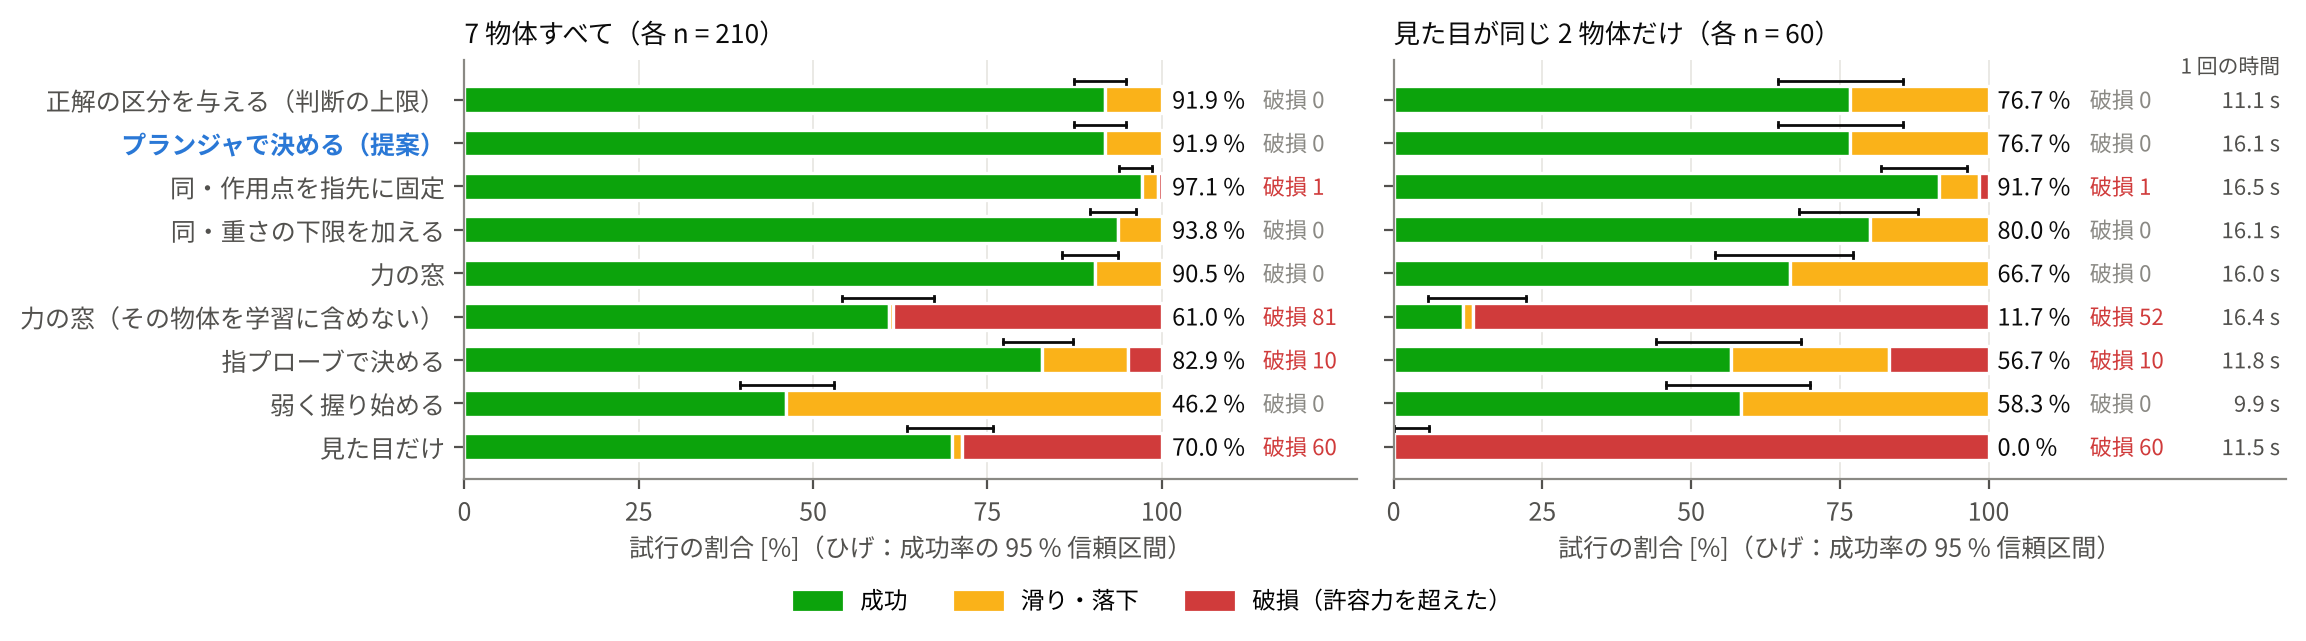
\includegraphics[width=0.98\textwidth]{fig_q2.png}
\caption{\textbf{Q2：目標把持力の決め方．}左：7 物体すべて．右：見た目が同じ 2 物体だけ．右端の数字は 1 回の平均時間．}
\label{fig:q2}
\end{figure*}

内圧表（区分ごとに二分探索で調整）は \V{q1.recipe.succ}\,\% で，区分が分かっていて，物体が調整に使ったものと同じ大きさなら，閉ループと同等の成功率に達する．
エンジンを替えても（\ref{sec:sim2sim} 節），筋肉がずれても（\ref{sec:robust} 節），閉ループとの差は小さかった．
閉ループの利点は，物体の大きさが調整時と違うときに，破損を減らせる点に出る．一方，大きく重い物では落下が増え，成功率は内圧表を下回った（\ref{sec:size} 節）．
したがって Q1 への答えは「推定した力の帰還だけで，基本 5 物体を破損 0・成功 \V{q1.learned.succ}\,\%で握れる（残りは落下）」であり，内圧表に対する利点は，調整時と条件が変わっても許容力を超えない点にある．

作用点を指先に固定すると，力を約 1 割小さく見積もり（推定値÷真値 \V{q1.tip.bias}），推定誤差は \V{q1.tip.mae}\,N に増える．その分強く握るので落下は減った（成功 \V{q1.tip.succ}\,\%，不一致の組 \V{t.q1.learned-learned_tip.ab}，$p_{\mathrm{Holm}}$ \V{t.q1.learned-learned_tip.p}）．許容力に余裕のない過熟の物体では，この偏りが破損になる（\ref{sec:q2} 節）．
真の力で帰還しても \V{q1.ideal.succ}\,\% で，推定値で帰還した学習モデルと変わらない．
残った失敗（豆腐の落下）は推定の誤差だけでは説明できない（真の力で帰還しても \V{q1.ideal.tofudrop} 件落ちた）．落ちた個体は摩擦が小さく重い側に偏る（摩擦係数÷質量と落下の相関は負）．PhysX ではどの方式でも豆腐を 1 つも落とさなかったので，豆腐の落下は箱の角と指先の接触のモデル化にも左右される（\ref{sec:sim2sim} 節）．






\subsection{Q2：見た目が同じ物体を見分けられるか}
\label{sec:q2}
7 物体×30 シードで，学習済みの分類器を使って閉ループで比べた（図\ref{fig:q2}）．
\begin{itemize}
\item \textbf{見た目だけ}：過熟の 2 物体をトマト・いちごとして 2.2\,N で握り，全数（60/60）潰した．
\item \textbf{弱く握り始める}：過熟いちごは運べた．しかし重い物は搬送中に落とした（成功 \V{q2.soft.succ}\,\%）．滑りは持ち上げの瞬間にしか判定できず，落下はその後に起きるので，強める機会がない．
\item \textbf{指プローブで決める}：見た目が同じ物体で \V{q2.finger.la}\,\% にとどまり，\V{q2.finger.la.cr} 回潰した（過熟を熟した方と見誤った）．
\item \textbf{プランジャで決める}：\V{q2.plunger.la}\,\% で，正解の区分を与えた上限（\V{q2.oracle.la}\,\%）に並んだ．指で決める方式との不一致の組は \V{t.q2.plunger-finger.la.ab}（$p_{\mathrm{Holm}}$ \V{t.q2.plunger-finger.la.p}）である．
\item \textbf{作用点を指先に固定}：力を 1 割ほど小さく見積もり，その分強く握る．落下は減り，見た目が同じ物体の成功は \V{q2.tip.la}\,\% で，点推定では R5 を満たした．ただし過熟いちごを \V{q2.tip.la.cr} 回潰した．回数の差は 1 件で，検定では判断できない（$p_{\mathrm{Holm}}$ \V{t.q2.plunger-plunger_tip.la.cr.p}）．それでも，許容力と目標の差が目標の 25\,\% しかない物体では，1 割の過小推定だけでこの余裕の 4 割を失う．成功率の高さは推定精度ではなく，力を約 1 割強く出す暗黙の安全率による．その一部は，推定を正しく保ったまま必要な物体にだけ目標を上げる重さの下限でも得られる（次項，\V{q2.mass.la} 対 \V{q2.tip.la}\,\%）．本研究は推定を正しく保ち，許容力との余裕を明示的に設計する方式を採った．
\item \textbf{重さの下限を加える}：推定は正しいまま，見た目の種類の名目の質量と摩擦から目標の下限を上げる（式\eqref{eq:massfloor}，\ref{sec:size} 節）．見た目が同じ物体の成功は \V{q2.mass.la}\,\%，全 7 物体で \V{q2.mass.succ}\,\%，破損 \V{q2.mass.cr}．過熟トマトの落下が \V{fail.plunger.tomato_overripe} 件から \V{fail.massv.tomato_overripe} 件に，豆腐が \V{fail.plunger.tofu} 件から \V{fail.massv.tofu} 件に減った．係数 $S$ は評価と同じ個体を含む試行で決めたので，参考の値である．
\item \textbf{力の窓}：学習に含めた物体では破損 \V{q2.fw.cr} 件だったが，見た目が同じ物体の成功は \V{q2.fw.la}\,\%（残りは落下）にとどまった．評価する物体を学習から除くと，破損は \V{q2.fwloo.cr} 件に増えた．
\end{itemize}
代償は時間で，1 回の把持は見た目だけで決める場合より平均 \V{q2.ct.delta}\,s 延びる（図\ref{fig:q2} 右端）．押す速さ 1\,mm/s が支配的で，速くしたときの判別精度は今後の課題である．



\subsection{Q3：生成データだけで判断を学習できるか}
\V{ds.n} 試行を 2 CPU で \V{ds.min} 分で生成し，全試行が検証器を通った．
区分の正解率（層化 5 分割交差検証）は，画像のみ \V{cv.vision}\,\%，画像＋指プローブ \V{cv.finger}\,\%，画像＋プランジャ \V{cv.plunger}\,\% だった．
画像のみでは，熟した方と過熟を区別できない．このデータだけで学習した分類器を Q2 の閉ループで使い，上の結果を得た．
なお，剛性の乱数（$\pm$20\,\%）では熟した方と過熟の範囲が重ならないので，\V{cv.plunger}\,\% は個体差がこの範囲に収まる場合の値である．また学習と評価は同じシミュレータの中で行っており，実物の画像とプランジャの波形への転移は確かめていない．人手なしで区分と成否のラベルが得られるのはシミュレータならではの利点で，実機では区分のラベルは得られず，成否のラベルにも破損の検出が要る．

\subsection{物理エンジンを替える}
\label{sec:sim2sim}
制御コアは変えず，指と物体の動力学だけを PhysX に替えた（図\ref{fig:q1} 右，各方式 $n=\V{px.n}$）．
PhysX のセルは同じ寸法・質量・関節剛性で USD に組み，スキンは接触点を指の座標に戻して 24 点に振り分けた．
同じシードは同じ個体なので，試行ごとに 2 つのエンジンを突き合わせられる．エンジンの差は動力学だけではない．真の把持力は，MuJoCo では接触点ごとの法線力の和，PhysX では指の節ごとの法線力ベクトルの和の大きさで，節の中で法線がそろわない分だけ後者が小さくなる．MuJoCo のスキン（touch センサ）は指先どうしやトレーとの接触も数えるが，PhysX では物体との接触だけを数えた．
\begin{itemize}
\item \textbf{成否}：学習モデルの閉ループは PhysX で \V{s2s.learned.px}\,\%（同じ 20 シードの MuJoCo では \V{s2s.learned.mj}\,\%），破損はどちらも 0 だった．成否と破損の組は \V{s2s.learned.same} の個体で一致した．両エンジンとも成功がほぼ全数なので，この一致数は偶然でもほぼ同じ値になる（Cohen の一致係数 $\kappa_{\mathrm C}=\V{s2s.learned.kappa}$）．
\item \textbf{判別力のある比較}：失敗の多い直線モデルでは，一致は \V{s2s.affine.same}，$\kappa_{\mathrm C}=\V{s2s.affine.kappa}$ で，いちごは PhysX でも全数潰れた．破損の有無は，直線モデル以外のすべての方式で 100 個体とも一致した．
\item \textbf{不一致}：全方式で \V{s2s.all.same} 組が一致し，不一致 \V{s2s.diff.n} 件のうち \V{s2s.diff.tofu} 件は，MuJoCo で落ちた豆腐を PhysX では運べたものである．PhysX ではどの方式でも豆腐を落とさなかった．直方体の角と指先の接触が，接触モデルの違いに最も敏感だった．
\item \textbf{力}：柔らかい 3 物体（いちご・豆腐・トマト）では，同じ個体のピーク力の差は中央値 \V{s2s.learned.rel.soft}\,\%（学習モデル）だった．硬い卵とボルトでは \V{s2s.learned.rel.stiff}\,\% 違った．
\end{itemize}
差の出どころを，力の時系列を残したシード 0 の 5 試行で位相ごとに調べた．
把持の位相の最大力は，5 物体とも 2\,\% 以内で一致した．
差が出るのは搬送の加減速の瞬間で，硬い卵とボルトでは MuJoCo の方が大きく（卵 4.1 対 2.9\,N，ボルト 5.1 対 3.3\,N），いちごでは PhysX に一瞬の山が出た（2.96\,N．破損の判定に使う 60\,ms 平均では許容力 3.0\,N 未満）．
硬い接触では，慣性力が出入りするときの力の山が，接触の減衰の扱い（MuJoCo のソフト拘束，PhysX のコンプライアント接触と TGS ソルバ）で変わるためと考えられる．
卵とボルトの値は許容力 25\,N の 1/4 以下で，判定は変わらない．
実行環境の GPU ドライバが Isaac Sim 5.0 の RTX 描画に対応していないため，PhysX は描画なしで計算し，動画は PhysX が計算した姿勢を MuJoCo の描画器で表示した．

\subsection{筋肉と指が想定とずれたら}
\label{sec:robust}
筋肉の 6 つの定数を，試行ごとに独立に最大 $\pm$10〜30\,\% ずらした（図\ref{fig:robust}，5 物体×10 シード，各 $n=50$）．
$\pm$30\,\% では，学習モデルの成功率は \V{rob.learned.30}\,\% に下がり，\V{rob.learned.30.cr} 回潰した．
空中較正（\ref{sec:decide} 節）を入れると，\V{rob.learnedcal.30}\,\% まで回復した（ずれなしは \V{rob.nominal.learned}\,\%）．破損は \V{rob.learnedcal.30.cr} 回残った．同じ条件の内圧表は成功 \V{rob.recipe.30}\,\%，破損 \V{rob.recipe.30.cr} 回だった．
空中較正は，指先どうしが触れる手前（曲げ 24°）までしか行えない．公称の筋肉では約 12\,kPa でここに達するので，把持に使う 15〜24\,kPa の差は最後に測った値で外挿している．このため，ずれがなくても空中較正は把持力をやや上げる（ピーク÷目標 \V{rob.nominal.learned.pk} → \V{rob.nominalcal.learned.pk}）．

指の曲げ剛性 $k_b$ のずれは，力の推定にそのまま比例して入る．$k_b$ が 25\,\% 硬いと，真の把持力は推定より約 25\,\% 大きくなる（ピーク÷目標の中央値が \V{rob.kb100.pk} から \V{rob.kb125.pk} へ）．
空中較正は空中で行うので，筋肉側の偏りしか取れず，$k_b$ のずれは残る．上の外挿の分だけむしろ広がる（空中較正ありで \V{rob.kb125cal.pk}，破損 \V{rob.kb125cal.cr} 回）．
逆に $k_b$ が 2 割柔らかいと力が足りず，落下で成功率は方式によって（図にない静特性の表を含む）\V{rob.kb080.min}〜\V{rob.kb080.max}\,\% に下がった．
実機では，ロードセルを一度押して $k_b$ を校正する手順が要る．

\begin{figure*}[t]
\centering
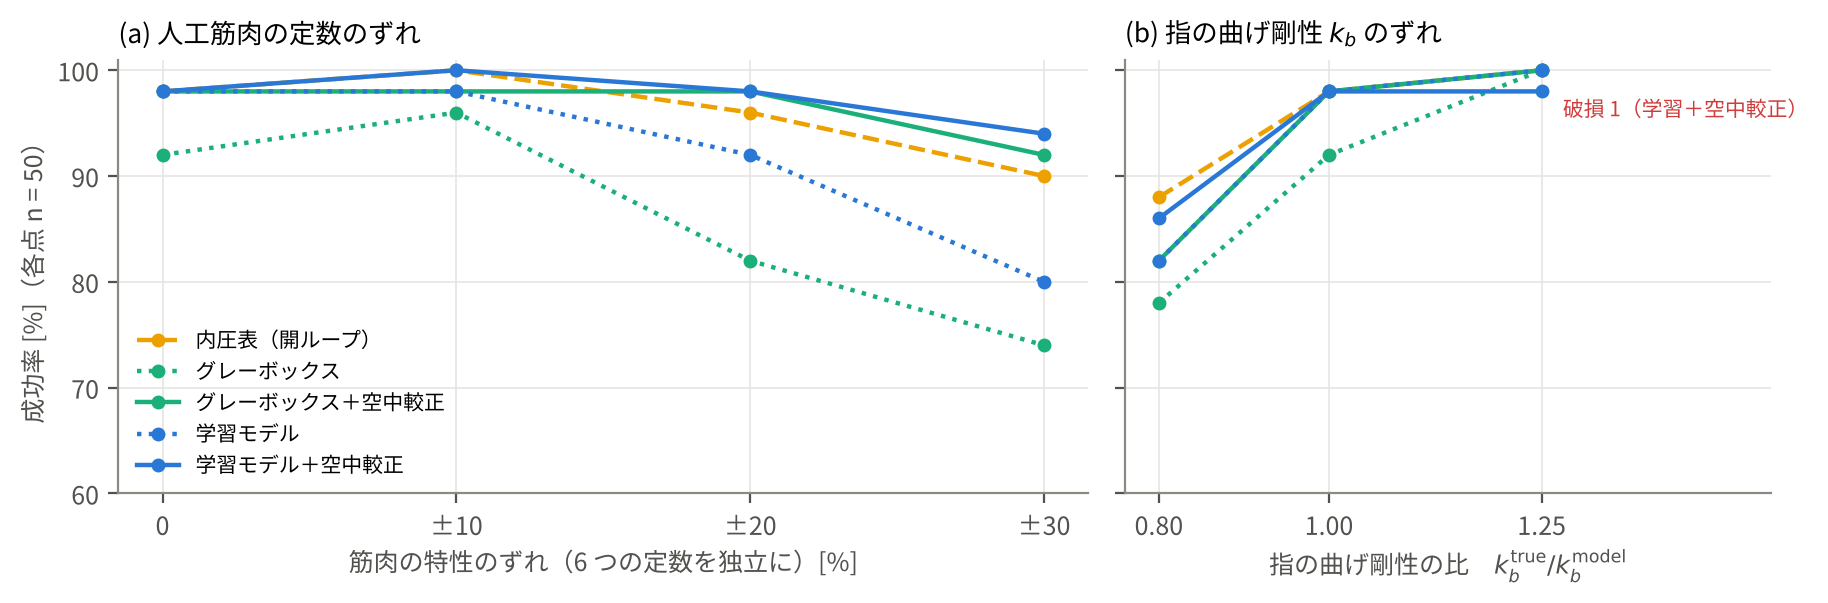
\includegraphics[width=0.86\textwidth]{fig_robustness.png}
\caption{\textbf{想定とのずれ．}(a) 人工筋肉の定数のずれ．(b) 指の曲げ剛性 $k_b$ のずれ．各点 $n=50$ で，Wilson 区間の幅はおよそ $\pm$10 ポイントある．破損の回数は本文に示す．}
\label{fig:robust}
\end{figure*}

\subsection{物体の大きさが変わったら}
\label{sec:size}
内圧表は，調整に使った大きさの物体でしか力を保証しない．
そこで，脆い 3 物体と過熟中玉トマトの寸法を 0.8 倍と 1.2 倍にした（質量は 3 乗，接触剛性・摩擦・許容力はそのまま，個体は同じシード）．
両方式に正しい区分を与え，判断の影響は除いた（表\ref{tab:size}）．
\begin{itemize}
\item \textbf{力}：内圧表のピーク÷目標の中央値は，0.8 倍で \V{ss.recipe.0.8.pk}，1.2 倍で \V{ss.recipe.1.2.pk} だった．小さい物には指が深く閉じてから触れるので，曲げの不足が小さく，力も小さい．大きい物はその逆になる．閉ループは \V{ss.learned.1.2.pk}〜\V{ss.learned.0.8.pk} で，大きさによらない．
\item \textbf{小さい物}：閉ループは \V{ss.learned.0.8.succ} で全数を運んだ．内圧表は \V{ss.recipe.0.8.succ} で，失敗はすべて過熟トマトの落下だった．
\item \textbf{大きい物}：内圧表は過熟トマトを \V{ss.recipe.1.2.cr} 回潰した（ピークは許容力の 1.01〜1.05 倍で，うち 8 回はその後に落とした）．閉ループは 1 回も潰さなかったが，成功は \V{ss.learned.1.2.succ} と内圧表（\V{ss.recipe.1.2.succ}）を下回った．大きい豆腐（質量 1.7 倍）は \V{ss.learned.1.2.tofu.succ}，大きい過熟トマトは \V{ss.learned.1.2.tomato_overripe.succ} しか運べず，残りは搬送中に落とした．内圧表は大きい物ほど強く握るので落下は減るが，許容力の幅が狭い過熟トマトではその強さが破損になる．
\end{itemize}
物体が大きくなって変わるのは，潰さない力の上限ではなく，落とさない力の下限である．下限は質量にほぼ比例し，寸法の 3 乗で増える．
準静的に，接触の法線が水平なら，摩擦で支えられる力の上限は $\mu\sum_f F_f=\mu F$ なので，保持には $\mu F\ge m\,|\bm g+\bm a|$ が要る．
そこで摩擦の余裕を $M=\mu F^*/\{m(g+a)\}$ と定義する（$a=0.9$\,m/s$^2$ は搬送の最大加速度．加速度は水平なので $|\bm g+\bm a|=\sqrt{g^2+a^2}$ が正しく，$g+a$ は約 9\,\% 保守側）．$M$ が 1 を大きく超えないと落ちるのは，接触の法線が水平でないこと，搬送中の慣性と回転，指 3 本の力の偏りのためである．
閉ループの目標に，大きさから推した重さで決まる下限（この試験では寸法比は真値を与えた） $M\ge S$ を加えた．
\begin{equation}
F^* = \min\Bigl(\max\bigl(H_{\mathrm t}(c),\ S\,\hat m(g+a)/\hat\mu\bigr),\ \V{ss.mass.cap}\,H_{\mathrm{lim}}(c)\Bigr)
\label{eq:massfloor}
\end{equation}
$H_{\mathrm t}(c)$ と $H_{\mathrm{lim}}(c)$ は取扱い表の目標と区分の許容力（大きさの試験では正しい区分 $c$，Q2 では推定した区分 $\hat c$ を使う），$\hat m$ は種類ごとの名目の質量×寸法比の 3 乗，$\hat\mu$ は種類ごとの名目の摩擦係数で，個体のばらつきは知らない．上限を許容力の 0.85 倍としたのは，閉ループのピークが多くの試行で目標の約 1.1 倍に収まるため（0.85×1.1 < 1）である．ただし 1.2 倍の過熟トマトでは，ピークが目標の 1.23 倍に達して潰れた試行が 1 件あった（シード 19）．
経験係数 $S=\V{ss.mass.safety}$ は等倍の物体だけから決めた（形の問題で落ちる過熟いちごを除くと，トマト（$M=2.9$）は落ちず，豆腐（2.3）は 1 割，過熟トマト（2.0）は 3 割落ちた）．
等倍では過熟トマトの目標が 1.55 から \V{ss.mass.F.tomato_overripe.1}\,N に上がり（下限 1.92\,N が上限で頭打ちになる），成功は \V{ss.learned.1.succ} から \V{ss.mass.1.succ} になった（$S$ を決めたのと同じ試行なので，この改善は甘めに出る）．
1.2 倍では \V{ss.mass.1.2.succ}（破損 \V{ss.mass.1.2.cr}）にとどまる．大きい過熟トマトに要る下限は \V{ss.mass.Fmin.tomato_overripe.1.2}\,N で許容力 2.0\,N を，大きい豆腐の \V{ss.mass.Fmin.tofu.1.2}\,N は区分の許容力 3.0\,N を超える．この把持方式では，潰さず落とさない力の範囲が存在しない．
窓がないことは握る前に計算で分かるので，実際の工程では見送って別の把持（底を支える，包む）に回すのがよい．
図\ref{fig:window}に，大きさに対する力の窓を示す．閉ループが運べなかったのは，目標力（点線）が落とさない下限の帯に入った条件だけである．大きいトマトは下限の中心線より下でも \V{ss.learned.1.2.tomato.succ} を運んだので，$S=\V{ss.mass.safety}$ は丸い物には保守側である．

\begin{figure*}[t]
\centering
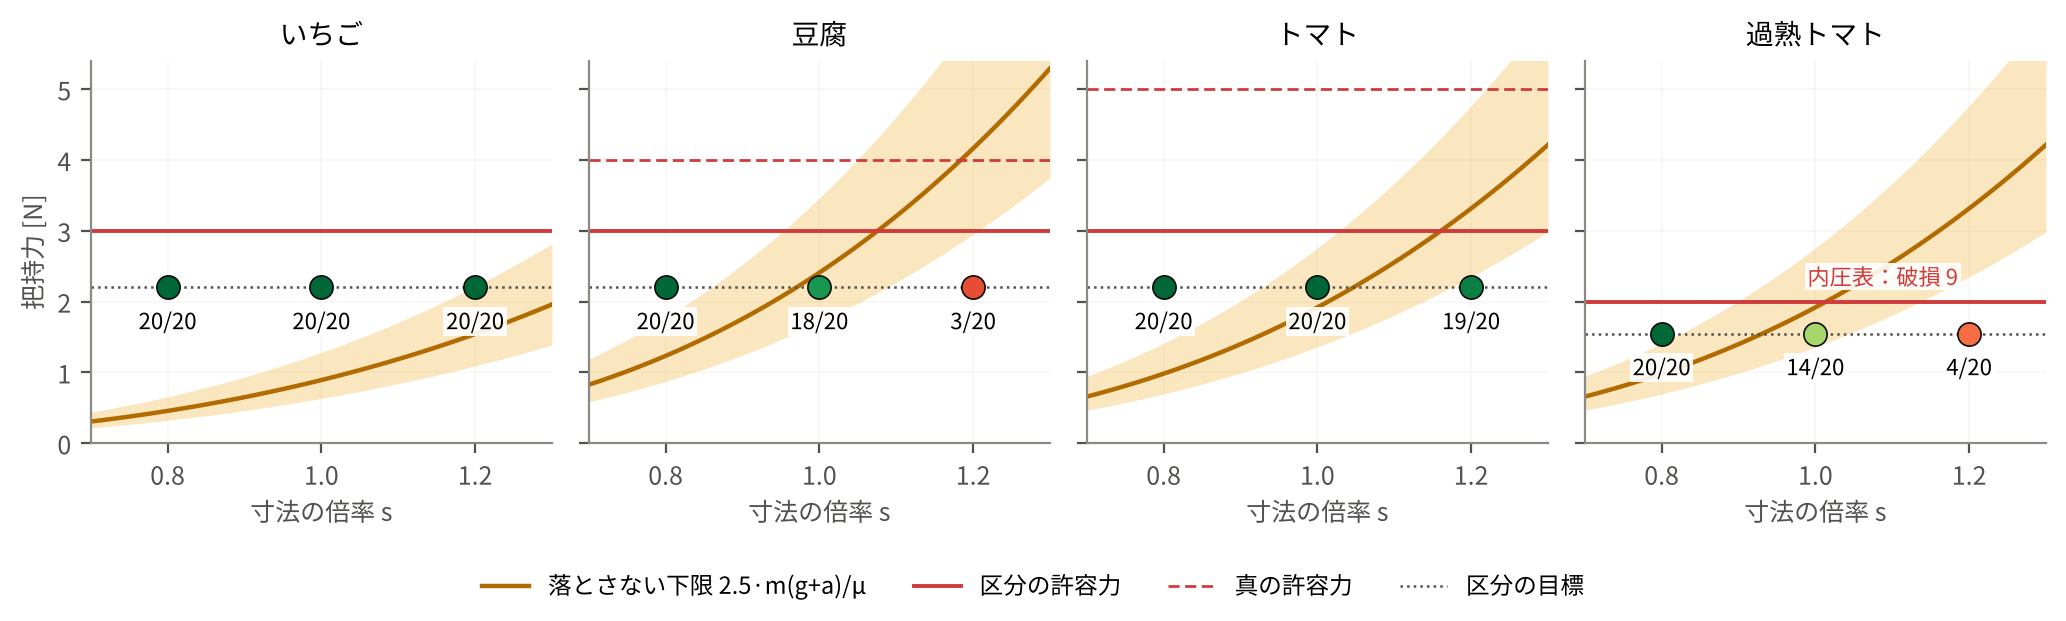
\includegraphics[width=0.95\textwidth]{fig_force_window.png}
\caption{\textbf{大きさに対する力の窓．}茶線は落とさない下限 $S\,m(g+a)/\mu$（名目の質量を寸法の 3 乗で増やす），帯は質量 $\pm$15\,\%・摩擦 $\pm$20\,\% の個体差の範囲．赤の実線は取扱い表の区分の許容力，破線は物体の真の許容力．横軸 $s$ は名目の寸法に対する倍率．点は閉ループ（学習モデル，区分の目標で握る）の成功数で，色は成功率（赤：0，黄：0.5，緑：1）．}
\label{fig:window}
\end{figure*}

\begin{table}[t]
\centering\small
\caption{大きさを変えた物体（4 物体 $\times$ \V{ss.n} シード，各 $n=80$）．成功（括弧内は破損）．ピーク÷目標は真の最大把持力と目標力の比の中央値．}
\label{tab:size}
\footnotesize\setlength{\tabcolsep}{2.2pt}
\begin{tabular}{@{}c cc cc c@{}}
\toprule
 & \multicolumn{2}{c}{内圧表（開ループ）} & \multicolumn{2}{c}{閉ループ・学習} & ＋重さの下限 \\
\cmidrule(lr){2-3}\cmidrule(lr){4-5}\cmidrule(l){6-6}
倍率 & 成功 & ピーク/目標 & 成功 & ピーク/目標 & 成功 \\
\midrule
0.8 & \V{ss.recipe.0.8.succ}（\V{ss.recipe.0.8.cr}） & \V{ss.recipe.0.8.pk} & \V{ss.learned.0.8.succ}（\V{ss.learned.0.8.cr}） & \V{ss.learned.0.8.pk} & \V{ss.mass.0.8.succ}（\V{ss.mass.0.8.cr}） \\
1.0 & \V{ss.recipe.1.succ}（\V{ss.recipe.1.cr}） & \V{ss.recipe.1.pk} & \V{ss.learned.1.succ}（\V{ss.learned.1.cr}） & \V{ss.learned.1.pk} & \V{ss.mass.1.succ}（\V{ss.mass.1.cr}） \\
1.2 & \V{ss.recipe.1.2.succ}（\textcolor{crit}{\V{ss.recipe.1.2.cr}}） & \V{ss.recipe.1.2.pk} & \V{ss.learned.1.2.succ}（\V{ss.learned.1.2.cr}） & \V{ss.learned.1.2.pk} & \V{ss.mass.1.2.succ}（\V{ss.mass.1.2.cr}） \\
\bottomrule
\end{tabular}
\end{table}

\subsection{開発に使っていないシードでの確認}
\label{sec:holdout}
最終の構成（筋肉モデル，取扱い表，分類器，空中較正）を固定し，シード \V{ho.seeds} で Q1 と Q2 を再実行した．
Q1 では，学習モデルの閉ループが成功 \V{ho.q1.learned.succ}\,\%・破損 \V{ho.q1.learned.cr}/\V{ho.q1.n}（シード 0〜29 では \V{q1.learned.succ}\,\%），内圧表が \V{ho.q1.recipe.succ}\,\%，直線モデルが \V{ho.q1.affine.succ}\,\%（破損 \V{ho.q1.affine.cr}）だった．
Q2 では，見た目が同じ 2 物体の成功が，見た目だけで決めると \V{ho.q2.prior.la}\,\%（破損 \V{ho.q2.prior.la.cr}），プランジャで決めると \V{ho.q2.plunger.la}\,\%（破損 \V{ho.q2.plunger.la.cr}），正解の区分を与えると \V{ho.q2.oracle.la}\,\% だった．重さの下限を加えた方式は \V{ho.q2.mass.la}\,\%（破損 \V{ho.q2.mass.la.cr}），作用点を指先に固定した方式は \V{ho.q2.tip.la}\,\%（破損 \V{ho.q2.tip.la.cr}）である．
主な結論（直線モデルだけが潰す，閉ループは破損 0，プランジャは見た目の判断の破損をなくし正解の区分の場合に並ぶ）は，未使用のシードでも変わらなかった．

\subsection{失敗の分析}
Q2 の失敗を，判断した区分と真の区分の関係で分けた（\texttt{metrics.json} の \texttt{failures}）．
見た目だけで決めた場合，失敗 \V{fail.prior.n} 件のうち \V{fail.prior.firmer} 件が「柔らかい物を硬い側に見誤って潰す」型だった．
プランジャで決めた場合，この型は \V{fail.plunger.firmer} 件で，失敗 \V{fail.plunger.n} 件はすべて落下である．
しかも \V{fail.plunger.n} 件は，正解の区分を与えた上限で失敗した \V{fail.oracle.tomato_overripe}＋\V{fail.oracle.strawberry_overripe}＋\V{fail.oracle.tofu} 件と同じ試行だった（共通 \V{fail.common} 件）．残る失敗は判断ではなく，握り方で起きている．
落下の中身は物体によって違う．摩擦の余裕 $M$（\ref{sec:size} 節）で比べた．
\begin{itemize}
\item \textbf{過熟トマト}（\V{fail.plunger.tomato_overripe} 件）：落とした個体は重く（中央値 \V{fail.mass.tomato_overripe.fail}\,g 対 \V{fail.mass.tomato_overripe.ok}\,g），摩擦が小さい（\V{fail.mu.tomato_overripe.fail} 対 \V{fail.mu.tomato_overripe.ok}）．余裕は \V{fail.margin.tomato_overripe.fail} 対 \V{fail.margin.tomato_overripe.ok} で，目標 1.55\,N では足りない個体がある．
\item \textbf{過熟いちご}（\V{fail.plunger.strawberry_overripe} 件）：余裕は \V{fail.margin.strawberry_overripe.fail} あり，力も目標に保たれたまま，搬送の途中で楕円体が指のあいだから押し出されて抜ける．把持の形の問題である．
\item \textbf{豆腐}（\V{fail.plunger.tofu} 件）：摩擦の小さい個体に偏る（$\mu$ の中央値 \V{fail.mu.tofu.fail} 対 \V{fail.mu.tofu.ok}）．
\end{itemize}
潰れは製品に残るが，落下はトレー上で検知すれば再把持できる．ただし，落とした食材を再利用できるかは工程の衛生基準による．
要求 R5（見た目が同じ物体の成功 85\,\%）は，提案の方式では点推定 \V{q2.plunger.la}\,\% で未達である．
重さの下限を加えると \V{q2.mass.la}\,\% まで上がり，未使用のシードでは \V{ho.q2.mass.la}\,\%（破損 \V{ho.q2.mass.la.cr}，Wilson 区間 \V{ho.q2.mass.la.ci}）と点推定で R5 を上回った（係数 $S$ はシード 0〜19 だけで決めたので，こちらは独立な検証である）．それでも過熟いちごの落下は残る．過熟いちごは力を上げる余地がなく（目標 1.2\,N，許容力 1.5\,N），把持の形（包む深さ，指の配置）を変える必要がある．

\section{限界}
\begin{enumerate}[label=(\roman*)]
\item 評価はすべてシミュレーションで，筋肉とセンサは仮定した特性のモデルである．実機の筋肉で同じ評価をするまで，学習モデルの利点（構造を知らなくてよいこと）は確かめられない．
\item 果実は剛体の外形と接触の柔らかさで近似した．局所的な変形と損傷の進行は扱っていない．許容力のうち，卵以外は文献の測定ではなく仮定である．接触剛性は 4\,mm の平型プローブの値を指の接触にそのまま当てた．実際の指のパッドと果実の接触は Hertz 型の非線形で，同じ弾性率（$E^*\approx375$\,kPa）で半径 22\,mm の球を指 1 本 0.73\,N で押すと接線剛性は約 2.4\,N/mm と，仮定の 1.6 倍になる．
\item 過熟の剛性の比（2.5）は仮定である．判別マップ（図\ref{fig:map}）で比への依存は示したが，実物の個体のばらつきは未測定である．
\item 物体の位置は，シミュレーションの真値を使った．
\item 指の曲げ剛性 $k_b$ のずれは，空中較正では補正できない．$k_b$ は内圧によらず一定と仮定したが，実際の空圧の指は内圧で硬くなる．
\item 模擬筋肉の履歴は，上昇と下降の枝のあいだを動く遊び（play）要素 1 つで表した．実物の小さなループの形は未確認で，筋肉モデルの比較の結果はこの形に依存しうる．
\item PhysX の評価は描画なしで，Q2 は MuJoCo だけで行った．
\item 提案方式の目標力は区分だけで決めた．重さの下限は \ref{sec:size} 節で試したが，名目の質量と摩擦を使うので，個体の重さと滑りやすさは見ていない．置く高さも計画値で決めており，手の中で物体が下がると台に押し付けうる．
\end{enumerate}

\section{まとめ}
見た目では分からない硬さの違いに対し，力センサのない柔らかい指で「押して確かめてから握る」仕組みを作り，物理を文献値に合わせた 2 つのエンジンで評価した．
不感帯・飽和と遅れを表す筋肉モデルと，触覚で作用点を求める推定によって，力センサなしで潰さず運べた（Q1）．推定の偏りは筋肉モデルの項と作用点の残差の 2 項でほぼ説明でき，センサの雑音の寄与は 1\,\% 以下だった．取扱い区分が既知で寸法が調整時と同じなら内圧表も同等の成功率を示すが，寸法が変わると破損が生じる．閉ループは破損を生じないが，大きく重い物体では落とさないための力の下限が支配的になる．
想定した雑音（曲げ 0.3°）では，指で触るだけでは文献の熟度差の範囲（比 1.3〜3.1）を見分けきれず，プランジャの判別精度は想定した雑音（2\,µm）と個体差（一様 $\pm$20\,\%）のもとでは個体差で決まることを判別マップで示した．硬さプランジャは見た目が同じ物体の成功率を 0\,\% から \V{q2.plunger.la}\,\% にし，重さの下限を加えると未使用のシードで \V{ho.q2.mass.la}\,\% に達した（Q2）．主な結論は，開発に使っていないシードでも変わらなかった．
判断は，人手なしで数分で作ったデータだけで学習できた（Q3）．
次は，シリコーン製の多室型（PneuNets 型）空圧曲げアクチュエータと M5Stack の空圧回路を製作し，人工筋肉 1 本の内圧と曲げ（カメラで計測）を記録してモデルを学び直し，筋肉モデルの評価（R1）を実機で確かめる．把持の評価は，グリッパを製作してから行う．

\begin{thebibliography}{99}\raggedright\small
\bibitem{moj2024} 法務省ほか，「飲食料品製造業分野における特定技能の在留資格に係る制度の運用に関する方針」，2024（https://www.moj.go.jp/isa/content/001416439.pdf）．
\bibitem{nikkei2025} 日経 BP，農林水産省 中小企業イノベーション創出推進事業 特集（惣菜盛付ロボット），2025（https://special.nikkeibp.co.jp/atclh/NXT/25/maff1029/）．
\bibitem{wilson1927} E. B. Wilson, ``Probable inference, the law of succession, and statistical inference,'' \textit{J. Am. Stat. Assoc.}, 22(158), 209--212, 1927.
\bibitem{black2024pi0} K. Black \textit{et al.}, ``$\pi_0$: A Vision-Language-Action Flow Model for General Robot Control,'' arXiv:2410.24164, 2024.
\bibitem{nvidia2025gr00t} NVIDIA, ``GR00T N1: An Open Foundation Model for Generalist Humanoid Robots,'' arXiv:2503.14734, 2025.
\bibitem{kawaharazuka2025} K. Kawaharazuka \textit{et al.}, ``Vision-Language-Action Models for Robotics: A Review Towards Real-World Applications,'' \textit{IEEE Access}, 2025 (arXiv:2510.07077).
\bibitem{romano2011} J. M. Romano, K. Hsiao, G. Niemeyer, S. Chitta, K. J. Kuchenbecker, ``Human-inspired robotic grasp control with tactile sensing,'' \textit{IEEE Trans. Robotics}, 27(6), 1067--1079, 2011.
\bibitem{spiers2016} A. J. Spiers, M. V. Liarokapis, B. Calli, A. M. Dollar, ``Single-grasp object classification and feature extraction with simple robot hands and tactile sensors,'' \textit{IEEE Trans. Haptics}, 9(2), 207--220, 2016.
\bibitem{scimeca2019} L. Scimeca, P. Maiolino, D. Cardin-Catalan, A. P. del Pobil, A. Morales, F. Iida, ``Non-destructive robotic assessment of mango ripeness via multi-point soft haptics,'' \textit{ICRA}, 2019.
\bibitem{magness1925} J.\,R. Magness, G.\,F. Taylor, ``An improved type of pressure tester for the determination of fruit maturity,'' \emph{USDA Circular}, 350, 1925.
\bibitem{shuto2026} Y. Shuto, D. V. Vargas, ``Sensorless damage-safe grasping,'' arXiv:2608.23983, 2026.
\bibitem{hwangbo2019} J. Hwangbo \textit{et al.}, ``Learning agile and dynamic motor skills for legged robots,'' \textit{Science Robotics}, 4(26), eaau5872, 2019.
\bibitem{thuruthel2019} T. G. Thuruthel, B. Shih, C. Laschi, M. T. Tolley, ``Soft robot perception using embedded soft sensors and recurrent neural networks,'' \textit{Science Robotics}, 4(26), eaav1488, 2019.
\bibitem{kuroki2024gendom} S. Kuroki \textit{et al.}, ``GenDOM: Generalizable One-shot Deformable Object Manipulation with Parameter-Aware Policy,'' \textit{ICRA}, 2024.
\bibitem{mosadegh2014} B. Mosadegh \emph{et al.}, ``Pneumatic networks for soft robotics that actuate rapidly,'' \emph{Advanced Functional Materials}, 24(15), 2163--2170, 2014.
\bibitem{howell2001} L. L. Howell, \textit{Compliant Mechanisms}, Wiley, 2001.
\bibitem{vursavus2017} K. K. Vursavuş, Z. Kesilmiş, Y. B. Öztekin, ``Nondestructive dropped fruit impact test for assessing tomato firmness,'' \textit{Chem. Eng. Trans.}, 58, 325--330, 2017.
\bibitem{krivanek2016} I. Křivánek, L. Máchal, L. Tunka, ``The effect of hen breeds on the egg response to the non destructive impact,'' \textit{Acta Univ. Agric. Silvic. Mendel. Brun.}, 64(4), 1191--1198, 2016.
\bibitem{todorov2012} E. Todorov, T. Erez, Y. Tassa, ``MuJoCo: A physics engine for model-based control,'' \textit{IROS}, 5026--5033, 2012.
\bibitem{sneddon1965} I. N. Sneddon, ``The relation between load and penetration in the axisymmetric Boussinesq problem for a punch of arbitrary profile,'' \textit{Int. J. Eng. Sci.}, 3(1), 47--57, 1965.
\bibitem{johnson1985} K. L. Johnson, \textit{Contact Mechanics}, Cambridge University Press, 1985.
\bibitem{mcnemar1947} Q. McNemar, ``Note on the sampling error of the difference between correlated proportions or percentages,'' \textit{Psychometrika}, 12(2), 153--157, 1947.
\bibitem{newcombe1998} R. G. Newcombe, ``Improved confidence intervals for the difference between binomial proportions based on paired data,'' \textit{Stat. Med.}, 17(22), 2635--2650, 1998.
\bibitem{holm1979} S. Holm, ``A simple sequentially rejective multiple test procedure,'' \textit{Scand. J. Stat.}, 6(2), 65--70, 1979.
\end{thebibliography}
\end{document}
